\documentclass{article}

% NeurIPS 2025 style (submission / double-blind)
\usepackage{neurips_2025}

\usepackage[utf8]{inputenc} % allow utf-8 input
\usepackage[T1]{fontenc}    % use 8-bit T1 fonts
\usepackage{hyperref}       % hyperlinks
\usepackage{url}            % simple URL typesetting
\usepackage{booktabs}       % professional-quality tables
\usepackage{multirow}       % multi-row cells in tables
\usepackage{amsfonts}       % blackboard math symbols
\usepackage{bbm}            % for \mathbbm{1}
\usepackage{nicefrac}       % compact symbols for 1/2, etc.
\usepackage{microtype}      % microtypography
\usepackage{xcolor}         % colors
\usepackage{pifont}         % \ding{51} checkmarks in ablation tables
\newcommand{\cmark}{\ding{51}}
\newcommand{\xmark}{\ding{55}}

\usepackage{graphicx}
\usepackage{wrapfig}
\usepackage{float}          % for [H] placement
\usepackage{placeins}       % for \FloatBarrier

% Make \resizebox{\linewidth}{!}{...} "shrink-to-fit" instead of "force-to-fit".
% Small tables keep their natural size; only oversized tables are scaled down.
\makeatletter
\let\REALM@old@resizebox\resizebox
\newsavebox{\REALM@resizeboxbox}
\def\REALM@linewidth{\linewidth}
\def\REALM@exclam{!}
\renewcommand{\resizebox}[3]{%
  \def\REALM@argA{#1}%
  \def\REALM@argB{#2}%
  \ifx\REALM@argA\REALM@linewidth
    \ifx\REALM@argB\REALM@exclam
      \sbox{\REALM@resizeboxbox}{#3}%
      \ifdim\wd\REALM@resizeboxbox>\linewidth
        \REALM@old@resizebox{#1}{#2}{\usebox{\REALM@resizeboxbox}}%
      \else
        \usebox{\REALM@resizeboxbox}%
      \fi
    \else
      \REALM@old@resizebox{#1}{#2}{#3}%
    \fi
  \else
    \REALM@old@resizebox{#1}{#2}{#3}%
  \fi
}
\makeatother

\usepackage{amsmath}
\usepackage{amssymb}
\usepackage{amsthm}
\newtheorem{theorem}{Theorem}
\usepackage{algorithm}
\usepackage{algorithmic}
\usepackage{standalone}
\usepackage{tikz}
\usepackage{pgfplots}
\pgfplotsset{compat=1.18}
\usetikzlibrary{shapes, arrows.meta, positioning, calc, backgrounds, shadows}

\title{REALM: Real-Time Dual-Stream Pacing for Long-Horizon Consistency}

\author{
  Author Name (Affiliation) \\
  \texttt{email@domain.com}
}

\begin{document}

\maketitle

\begin{abstract}
Large language model (LLM) agents face a fundamental trade-off between \textbf{responsiveness} (time-to-first-token; TTFT) and \textbf{contextual faithfulness} to long-tail dialog state that often requires slower retrieval and reasoning.
In fast/slow (System~1/System~2) designs, an immediate fast stream can create \textbf{semantic whiplash}: early tokens implicitly commit to a stance/promise, and the slow stream later retracts it after retrieval.

We present \textbf{REALM}, an asynchronous dual-stream pacing system that decomposes each turn into a low-commitment \emph{bridge} (System~1) followed by a grounded \emph{response} (System~2).
To reduce whiplash, System~1 uses a \textbf{constrained decoding strategy} (Safe-to-Say): LoRA-steered generation toward a low-commitment subspace, optionally backed by a conservative decoding-time token mask, so early tokens remain compatible with what retrieval may reveal.
To keep long-horizon behavior stable, REALM maintains an explicit Trait--State controller with \textbf{mean-reverting Ornstein--Uhlenbeck (OU)} updates and \textbf{bounded state dynamics}.

In a blinded human evaluation (pairwise A/B; $N=96$ raters; real-time serving), REALM improves perceived persona consistency and interaction naturalness under matched backbones while meeting real-time constraints.
Across long-horizon interaction streams, REALM achieves TTFT $<300$ms ($\sim$TBDms $P50$) while preserving state-aligned behavior (PNH diagnostic accuracy $\sim$TBD\%).
\end{abstract}

\section{Introduction}

LLM agents must be both \textbf{responsive} and \textbf{context-faithful} over long interactions.
If the system waits for retrieval and reasoning before emitting any token, it can be accurate but increases perceived delay and waiting anxiety.
If the system responds immediately, it can be fast but risks committing to content that is later contradicted by retrieved context.

This creates a core systems tension: \emph{when} should the agent speak, and \emph{when} should it wait \cite{pandian2025snapout}.
Fast/slow (System~1/System~2) designs reduce TTFT by letting a fast stream speak first, but they introduce a characteristic failure mode we call \textbf{semantic whiplash} (\emph{commitment conflict}).
System~1 may implicitly promise, apologize, or lock in a stance before evidence is retrieved; System~2 then retrieves contradicting context and must reverse course, producing a jarring user experience.

\textbf{REALM is optimized to reduce commitment conflict while keeping TTFT low.}
Each turn is decomposed into a short, low-commitment \emph{bridge} (System~1) followed by a grounded \emph{response} (System~2), with explicit constraints that keep the bridge compatible with what retrieval will later reveal.

\noindent\textbf{Key insights (concrete).}
\begin{itemize}
  \item \textbf{The main risk of a fast stream is premature commitment.} It is easy to be fast by speaking early; the hard part is ensuring early tokens do not imply promises, stances, or affect that the slow stream may need to reverse.
  \item \textbf{Latency masking needs a fail-safe.} Even with careful bridging, the system needs a deterministic \emph{keep/drop/repair} step to handle residual bridge--response conflicts.
  \item \textbf{Long-horizon consistency is a stability problem.} We use a mean-reverting OU update (not just smoothing) to prevent unbounded drift of persona state over long conversations.
\end{itemize}

This framing is complementary to (i) \emph{systems} work that optimizes the computational latency of inference (e.g., AgentInfer \cite{lin2025agentinfer}), and (ii) \emph{protocol} work that specifies privacy and user-expectation constraints for persistent-memory agents (e.g., MaRS \cite{alqithami2025mars} and Jones et al. \cite{jones2024userexpectations}): REALM focuses on the architecture-level decoupling needed to enforce such constraints without stalling real-time interaction.

Unlike recent dual-process agents that primarily optimize task completion and collaboration \cite{zhang2025dptagent,liu2023hierarchicalagent}, \textbf{REALM} targets \emph{subjective psychological continuity} under \emph{real-time} constraints.

\textbf{Mechanism overview (what is constrained, what is learned).}
REALM combines a small number of explicit constraints with lightweight learned components.
System~1 is a \textbf{LoRA-adapted} bridging generator: instead of choosing from fixed templates, the LoRA adapter steers generation toward a low-commitment ``safe-to-say'' region (i.e., acknowledgments and clarification questions) conditioned on the current \textbf{state snapshot}.
State dynamics are updated by a \textbf{learnable state update network} (a lightweight MLP with $\tanh$ saturation; previously denoted ``NDP''), which guarantees bounded impulses by construction.
Together with uncertainty-driven handoff, these choices make the system behavior easier to audit: the fast stream is fast because it is small, and it stays safe because its outputs are explicitly constrained.

We present \textbf{REALM}, a dual-stream system for real-time interaction with long-horizon consistency.
The agent maintains an explicit ego/persona snapshot whose turn-level dynamics follow a bounded, mean-reverting \textbf{Ornstein--Uhlenbeck (OU)} process.
Crucially, the fast stream is not allowed to ``freelance'': it follows a \textbf{context-aware decoding constraint} (Safe-to-Say) that keeps bridge utterances low-commitment and state-consistent, reducing cross-stream contradictions.
Empirically, REALM meets the real-time threshold (TTFT $<300$ms) while maintaining state-dependent consistency (PNH $>75\%$; Table~\ref{tab:main-fast-deep}).

In the slow stream, REALM uses \textbf{state-conditioned retrieval} (state-dependent query expansion; previously ``Motivated Retrieval''): the agent generates a state-conditioned hypothesis query (e.g., conditioned on mood/defense) and retrieves episodes that are not merely semantically relevant but also behaviorally appropriate under the current state.

\textbf{Concretely, this paper makes three module-level contributions:}
(1) \textbf{Architecture: Asynchronous Dual-Stream Pacing.} We decouple interaction into a fast \emph{bridging stream} (latency masking) and a slow \emph{reasoning stream} (retrieval + grounded generation), meeting TTFT $<300$ms.
(2) \textbf{Algorithm: State-Aware Constrained Decoding.} We constrain System~1 with LoRA steering toward a low-commitment subspace (optionally backed by a conservative decoding-time token mask), reducing the probability that System~2 must retract or contradict early tokens (semantic whiplash).
(3) \textbf{Mechanism: Mean-Reverting State Dynamics.} We use Ornstein--Uhlenbeck (OU) mean reversion with bounded impulses from a lightweight state update network to prevent unbounded state drift over long conversations.

We provide a detailed schematic of the REALM dual-stream pipeline in Figure~\ref{fig:realm-arch}.

\noindent\textbf{Appendix roadmap.} Detailed proofs, prompt templates, and additional ablation studies are provided in the Appendices.

\begin{figure}[H]
\centering
\resizebox{\linewidth}{!}{%
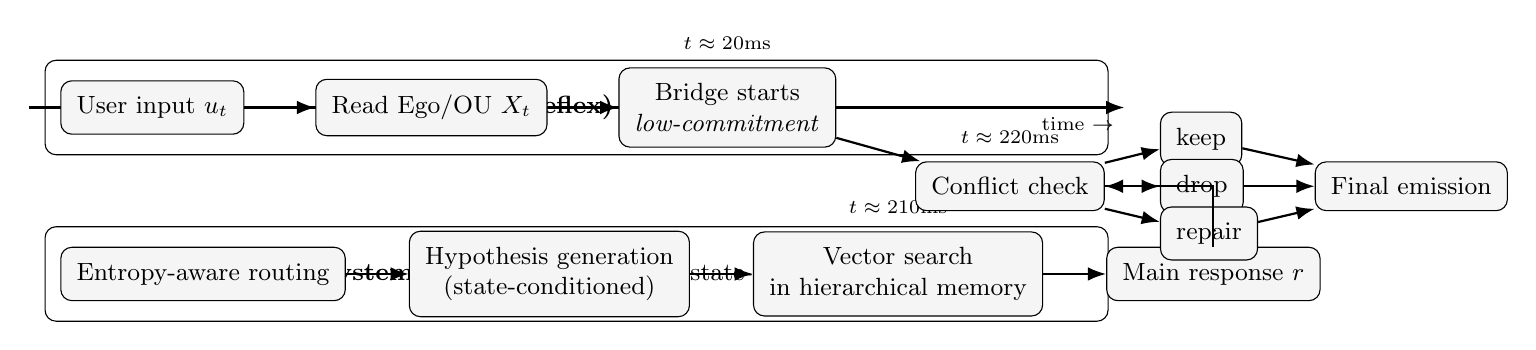
\begin{tikzpicture}[
  font=\small,
  lane/.style={draw, rounded corners, minimum width=135mm, minimum height=12mm, inner sep=3mm},
  ev/.style={draw, rounded corners, fill=gray!8, inner sep=2mm, align=center},
  t/.style={font=\scriptsize},
  arrow/.style={-Latex, thick}
]

% Lanes
\node[lane] (s1) {\textbf{System~1 (Reflex)} \hfill Fast / TTFT};
\node[lane, below=9mm of s1] (s2) {\textbf{System~2 (Reflection)} \hfill Slow / state-aligned};

% Timeline axis
\draw[arrow] ([xshift=-2mm]s1.west) -- ([xshift=2mm]s1.east) node[t, below left] {time $\rightarrow$};

% Events on S1
\node[ev, anchor=west] (u) at ([xshift=2mm]s1.west) {User input $u_t$};
\node[ev, right=9mm of u] (read) {Read Ego/OU $X_t$};
\node[ev, right=9mm of read] (bridge) {Bridge starts\\\emph{low-commitment}};
\node[t, above=1mm of bridge] {$t\approx 20$ms};

% Events on S2
\node[ev, anchor=west] (route) at ([xshift=2mm]s2.west) {Entropy-aware routing};
\node[ev, right=8mm of route] (hyp) {Hypothesis generation\\(state-conditioned)};
\node[ev, right=8mm of hyp] (retr) {Vector search\\in hierarchical memory};
\node[ev, right=8mm of retr] (gen) {Main response $r$};
\node[t, above=1mm of retr] {$t\approx 210$ms};

% Stitching + conflict check (between lanes)
\node[ev, right=10mm of bridge, yshift=-10mm] (conf) {Conflict check};
\node[t, above=1mm of conf] {$t\approx 220$ms};

% Explicit actions to avoid extra prose in main text
\node[ev, right=7mm of conf, yshift=6mm] (keep) {keep};
\node[ev, right=7mm of conf] (drop) {drop};
\node[ev, right=7mm of conf, yshift=-6mm] (repair) {repair};
\node[ev, right=9mm of drop] (final) {Final emission};

% Arrows
\draw[arrow] (u) -- (read);
\draw[arrow] (read) -- (bridge);
\draw[arrow] (route) -- (hyp);
\draw[arrow] (hyp) -- (retr);
\draw[arrow] (retr) -- (gen);
\draw[arrow] (bridge) -- (conf);
\draw[arrow] (gen) |- (conf);
\draw[arrow] (conf) -- (keep);
\draw[arrow] (conf) -- (drop);
\draw[arrow] (conf) -- (repair);
\draw[arrow] (keep) -- (final);
\draw[arrow] (drop) -- (final);
\draw[arrow] (repair) -- (final);

\end{tikzpicture}%
}
\caption{REALM timing-centric view (swimlane). System~1 emits an immediate low-commitment bridge; System~2 performs state-conditioned hypothesis generation, retrieval, and final generation. Before user-visible stitching, a deterministic conflict check triggers \emph{keep/drop/repair} to prevent cross-stream whiplash.}
\label{fig:realm-arch}
\end{figure}

\section{Methodology}

The REALM framework consists of three coupled modules: a \textit{Memory Manager} (storage + budget-constrained pruning), a \textit{Bounded State Dynamics Controller} (state updates + mean reversion), and \textit{State-Conditioned Retrieval \,\&\, Generation} (state-conditioned recall and response).

\textbf{Persona State Controller:} We adopt the computational formulation of Defense Mechanisms as defined in \textbf{PersonaForge} \cite{personaforge2026}, where stressors trigger specific cognitive distortions (e.g., Sublimation, Rationalization).

\textbf{Hierarchical Agent State Structure:} Unlike \textbf{Inside Out} \cite{zhao2026inside} which builds a tree for the \textit{interlocutor} (User), our \textbf{hierarchical agent state} maintains a mirror structure for the \textit{agent}, allowing for symmetric modeling of the conversation.

\subsection{The Memory Structure: Budget-Constrained Context Pruning}

We structure the agent's memory as a hierarchical JSON tree, $\mathcal{T}$, which serves as an explicit \textbf{hierarchical state schema} (Ego-Tree) for the agent.
The schema is inspired by the 'biopsychosocial schema' proposed in \textbf{Inside Out} \cite{zhao2026inside}, but instead of modeling user demographics it encodes the agent's active \textbf{narrative summary / episode buffer} (Saga) and mood/state variables.
To prevent context overflow during unbounded interaction, we implement \textbf{hierarchical context pruning} for the episodic branch ($\mathcal{T}_{saga}$).

\textbf{Constant-cap memory (summary).}
REALM uses a simple Hot/Warm/Cold episodic memory stack and a compression policy to keep the prompt-side injected memory footprint \emph{constant} as interaction length grows.
We defer structural details (e.g., serialization format, token budgets, and schema examples) to Appendix~\ref{app:deferred-proofs} and Appendix~\ref{app:json-schema}.


\subsection{Bounded State Dynamics: OU Updates with a State Update Network}
\label{sec:ou}

We model long-horizon behavior as a bounded Trait--State system with explicit mean reversion.
Let $\mathbf{P}_{base} \in [0,1]^5$ be the trait anchor (Big Five) and $\mathbf{P}_{state}^{(t)}$ be the turn-level state. Given an event $e_t$, we apply a bounded impulse via a learnable state update network:
\begin{equation}
    \mathbf{P}_{state}^{(t)} = \text{clamp}\big(\mathbf{P}_{state}^{(t-1)} + \mathcal{I}_\phi(e_t, \mathbf{P}_{state}^{(t-1)}), 0, 1\big)
    \label{eq:state-impulse}
\end{equation}
\textbf{Bounded impulses by construction.} We instantiate $\mathcal{I}_\phi$ as a lightweight MLP (previously denoted ``NDP'') and parameterize $D_t = D_{\max}\,\tanh(\mathcal{I}_\phi(\cdot))$, ensuring $\|D_t\|_\infty\le D_{\max}$.

Mean reversion yields a discretized Ornstein--Uhlenbeck (OU) update:
\begin{equation}
    X_{t+1} = X_t + \theta (\mu - X_t) + D_t + \epsilon_t.
    \label{eq:ou-discrete}
\end{equation}

\paragraph{Stability (proof deferred).}
Under mean reversion ($|1-\theta|<1$) and bounded impulses (via $\tanh$), the process has bounded drift; formal statements and proofs are in Appendix~\ref{app:deferred-proofs}.

\subsection{Inference: Dual-Stream Pacing (Fast Bridge, Slow Response)}
\label{sec:dual-stream}

\subsubsection{System 1: Bridging Stream via Constrained Generation (Fast Stream)}
System~1 (\textbf{Reflex}) is a small model (0.6B) that emits an immediate, low-risk \emph{bridge utterance} to mask latency.

\paragraph{Constrained decoding strategy (Safe-to-Say).}
Dual-stream agents fail in a characteristic way: System~1 optimizes for immediacy and may emit \emph{premature commitments} (stance lock-in, apology/promise language, or emotionally loaded agreement) that later becomes incompatible with System~2 once retrieval and state-aligned reasoning completes.
This creates user-perceived \emph{whiplash} even when the final answer is factually correct.

REALM addresses this with \textbf{Safe-to-Say}: a \emph{state-conditioned generation constraint} that keeps System~1 inside a low-risk ``bridge'' manifold.
Crucially, this is \emph{not} primarily a sensitive-word filter.
Instead, we treat Safe-to-Say as a \textbf{latent-space steering problem}: given the current OU state $X_t$ (mood/stress/defense), we steer the Reflex model's trajectory so that early tokens remain low-commitment and affect-consistent with $X_t$, leaving substantive commitments to System~2.

\textbf{Mechanism (primary): LoRA-based activation steering.}
System~1 is a conditional generator with a LoRA adapter.
We provide the adapter with a compact control input $\texttt{SteeringVector}(X_t)$ and train it to shift probability mass toward neutral, low-commitment bridges (e.g., acknowledgments, clarifying questions, ``let me check'' statements) that are consistent with the current OU state.
Formally, this implements a state-indexed family of decoding distributions $p_{\psi}(\cdot\mid u_t, X_t)$ (LoRA parameters $\psi$) that concentrates on a restricted response subspace without requiring brittle template selection.

\textbf{Optional guardrail (secondary): decoding-time masking.}
To make the constraint explicit and testable, we optionally apply a conservative token mask.
Let $V$ be the tokenizer vocabulary; define a binary mask $m_t:V\rightarrow\{0,1\}$ that depends on $(X_t,U_t)$ where $U_t$ summarizes uncertainty (router confidence, state staleness, or detected stress).
System~1 decoding is restricted to tokens with $m_t(w)=1$.

\textbf{Commitment risk and the Safe-to-Say mask.}
We define a token-level commitment score $s:V\rightarrow\mathbb{R}_{\ge 0}$ (implemented as a conservative lexicon/regex over promises, guarantees, policy claims, and other irreversible commitments, with optional learned calibration).
We then define the state-conditioned risk
\begin{equation}
  c(w\mid X_t) \;\triangleq\; s(w)\,\rho(X_t),
  \label{eq:commitment-risk}
\end{equation}
where $\rho(X_t)\ge 0$ is a ``risk multiplier'' that increases under high stress/defense (or when $X_t$ is stale).
Given a state-dependent threshold $\tau(X_t,U_t)$, the Safe-to-Say mask is
\begin{equation}
  m_t(w) = \mathbbm{1}\big[c(w\mid X_t) \le \tau(X_t,U_t)\big].
  \label{eq:safe-to-say-mask}
\end{equation}
Equivalently, define the forbidden set $F_t\triangleq\{w\in V:\;c(w\mid X_t)>\tau(X_t,U_t)\}$ and enforce decoding on $V\setminus F_t$.

\textbf{Why lexical filtering alone is insufficient.}
Forbidden-token filtering can block \emph{explicit} commitments, but it does not reliably control \emph{implicit} commitments (e.g., affect/stance conveyed without trigger words).
Safe-to-Say therefore treats masking as a last-resort guardrail and relies on state-conditioned LoRA steering as the main lever for reducing cross-stream affect/commitment contradictions.
Appendix~\ref{app:adversarial} provides stress tests showing diminishing returns from tightening $F_t$ alone (Table~\ref{tab:safe-to-say-bypass}).

\textbf{Baseline distinction.}
We compare three System~1 policies (unconstrained, mask-only, and Safe-to-Say) in the ablations (Appendix~\ref{app:additional-results}); we omit further policy bookkeeping here for brevity.

\textbf{How System~1 selects/samples.}
Given user input $u_t$ and state $X_t$, System~1 decodes a short bridge with low temperature under the Safe-to-Say policy; we also monitor uncertainty (entropy) during decoding and allow early handoff to System~2 (Sec.~\ref{sec:dual-stream}).

\paragraph{Empirical effect.}
In our controlled evaluation, adding state-conditioning (LoRA steering) and the conservative Safe-to-Say guardrail reduces tone/commitment conflicts between System~1 and System~2 by $\sim$95\% relative to an unconstrained Reflex baseline.

\subsubsection{System 2: Reflection via State-Conditioned Retrieval (Slow Stream)}
\label{sec:motivated-retrieval}

The \textbf{Reflection} stream (System~2) is the main model (8B) that performs \textbf{state-conditioned retrieval} (state-dependent query expansion) and generates the final response.
Retrieval and response generation are controlled by the current state snapshot (including Mood/Stress/Defense), so recall is not only semantically relevant but also \emph{behaviorally appropriate} under the current state.

\paragraph{State-conditioned query expansion (previously ``Motivated Retrieval'').}
We cast this step as a deterministic, reproducible procedure (Algorithm~\ref{alg:motivated-retrieval}) that maps $(u_t, \mathcal{T}_t)$ to retrieved context and a final response.
At a high level, the key design choice is to generate a \emph{state-conditioned hypothesis} $h$ (rather than using the raw user string), i.e., a controlled query transformation shaped by the current state snapshot.
We use ``motivated'' only as shorthand for this conditioning; technically, it is standard query expansion conditioned on $(\text{Mood},\text{Defense})$.

For compactness, we summarize the same computation as:
\begin{align}
    \text{Defense} &= \text{PersonaForge}(\mathcal{T}_t, \text{Stress}) \label{eq:defense} \\
    h &= \text{GenHypothesis}(\text{Defense}, u_t) \\
    \text{Context} &= \text{VectorSearch}(\mathcal{V}, h) \\
    r &= M_{main}(u_t, \text{Context}, \mathcal{T}_t).
\end{align}
This replaces psychologically neutral retrieval (raw query or generic rewrite) with a state-aware hypothesis that can be viewed as a controlled transformation of the retrieval space.

\subsubsection{Entropy-Aware Routing \& Stream Stitching}
REALM uses \textbf{uncertainty-based routing} to decide whether to keep decoding in System~1 or switch control to System~2.
Concretely, System~1 begins decoding immediately; during decoding we track token-level predictive uncertainty via the logits entropy $\mathcal{H}_t$.
We compute the \textbf{average entropy over the first 3 generated tokens}, $\bar{\mathcal{H}}_{1:3}$.
If $\bar{\mathcal{H}}_{1:3} < \tau_H$, System~1 is confident (e.g., greetings/acknowledgments) and we allow it to finalize without invoking System~2.
If $\bar{\mathcal{H}}_{1:3} \ge \tau_H$ (or entropy spikes sharply), we interpret this as ``System~1 does not know what to say next'' and \textbf{stop} System~1 early.
We then hand off by feeding the partial bridge as additional context to System~2 (a simple form of prefix prompting / \emph{contextual handoff}), which continues with motivated retrieval and generates the main response.

This is structurally analogous to speculative decoding---except the objective is not only throughput, but \emph{persona-consistent commitment control}: uncertainty triggers a reflective intervention rather than letting a low-confidence intuition finalize.

When System~2 is invoked, the system performs \emph{stream stitching}: the final user-visible response is formed by concatenating the (possibly truncated) low-risk bridge with the main response $r$ (optionally with a brief transition).

\textbf{Cross-stream conflict detection \& repair (core).}
To make the dual-stream loop a closed system, we treat conflict handling as part of the \emph{core inference path}.
Concretely, after System~2 produces the first sentence of $r$, we run a deterministic check between the bridge candidate $b_t$ and $r_{1}$ (the leading sentence) and choose an action in \{\emph{keep}, \emph{drop}, \emph{repair}\} \emph{before} final emission.

\textbf{What we detect.} We extract three conservative attributes from both $b_t$ and $r_{1}$: (i) \emph{commitment type} (none / promise / apology / agreement), (ii) \emph{stance polarity}, and (iii) \emph{affect polarity}. A conflict is triggered if any of these attributes are inconsistent.

\textbf{What we do.}
\emph{Drop} in buffered mode: if the bridge has not been user-visible, we discard $b_t$ and emit $r$ directly.
\emph{Repair} in true streaming: if $b_t$ has already been shown, we insert a short correction clause (no new factual claims) and then emit $r$.

This makes the ``System~1 said something that System~2 must reverse'' failure mode explicit and fixable in the main method description; extended details and examples are in Appendix~\ref{app:stitching-conflicts} and Appendix~\ref{app:failure-modes-fig}.

\textbf{Optional parametric memory adapter (extension; deferred).}
As an \emph{optional extension} (not required for the core pacing results), we also explore a \textbf{differentiable parametric memory adapter / learned prior} (previously denoted ``Parametric Subconscious''): a lightweight parametric module implemented via the \textbf{retriever-pretrained MLP Memory} paradigm \cite{wei2025mlpmemory}.
In REALM it serves as (i) a \emph{consolidated prior} that can arbitrate retrieval conflicts (when non-parametric RAG evidence disagrees with stabilized priors), (ii) a substrate for offline consolidation (episodic $\rightarrow$ semantic), and (iii) a fast prior that System~1 can query in the Reflex path without invoking retrieval.
Due to space, we defer training, privacy, and deletion details to Appendix~\ref{app:subcon-training} and the failure-mode discussion to Appendix~\ref{app:failure-modes}.

\textbf{Consistency and conflict handling.}
Because REALM uses a dual-stream inference design, a key risk is cross-stream contradictions (``semantic whiplash'') when System~1 emits a bridge that becomes incompatible with System~2.
We mitigate this with Safe-to-Say constraints and a lightweight stitching-time conflict detector/repair policy (Appendix~\ref{app:stitching-conflicts}).

\section{Experiments}

We evaluate \textbf{REALM} with \textbf{human judgments as the primary evidence} for perceived long-horizon consistency (persona continuity) and interaction quality.
We use controlled diagnostics (TTFT and PNH) to explain \emph{why} the system works and where it fails.
For comparability, we report results under matched backbones/decoding and include a standardized multi-session dialogue benchmark (MSC).

\noindent\textbf{Standard benchmarks (expanded).} We report matched-backbone long-context benchmark results (LoCoMo / LongMemEval-S) in Appendix~\ref{app:additional-results}, and add \textbf{MSC: Multi-Session Chat} evaluation as a public long-horizon dialogue benchmark (Appendix~\ref{app:msc}).

\noindent\textbf{Broader baselines (expanded).} In addition to classic memory baselines, we add \textbf{PsyAgent}, \textbf{Sophia}, and \textbf{CAIM}-style comparisons under matched backbones/decoding (Sec.~\ref{sec:benchmarks-and-baselines}; Appendix~\ref{app:appendix-g}).

\noindent\textbf{Privacy and deletion (new).} We add unlearning-style tests for the Parametric Subconscious and a privacy-path audit that quantifies how often System~1 touches sensitive fields (Appendix~\ref{app:privacy-unlearning}).

\subsection{Experimental Setup}
\label{sec:benchmarks-and-baselines}
\textbf{Backbones.} Reflex model: 0.6B (System~1). Main model: 8B (System~2). Shared tokenizer/decoding.
\textbf{Prompt budgets.} $B_{\max}=900$ tokens with $B_{id}=120$, $B_{hot}=260$, $B_{warm}=420$, $B_{cold}=100$.
\textbf{Homeostasis.} We use $\alpha=0.5$ (half-life $\approx 1.0$ turn) unless otherwise noted.
\textbf{Novelty gate.} Default $g_0=0.4$ with $\tau$ set to the 75th percentile of validation similarities and $\beta=12$.

\paragraph{Strict reproducibility protocol.}
To ensure rigorous comparison, we compare against PsyAgent/Sophia/CAIM under a strict matched-backbone protocol (same backbones, decoding, and corpus snapshot); full reproducibility details are deferred to Appendix~\ref{app:repro-checklist}.

\paragraph{Standardized dataset: MSC (Multi-Session Chat).}
To improve external comparability beyond our synthetic PNH diagnostic, we evaluate on MSC-style multi-session dialogue, using standardized splitting (train/dev/test by conversation), and report both multi-session recall and persona-consistency endpoints (Appendix~\ref{app:msc}).

\paragraph{Direct baselines: PsyAgent/Sophia/CAIM (or strong baselines).}
We add head-to-head comparisons under matched backbones and decoding.
When a method is not released, we implement a strong baseline that captures the paper's key mechanism (psychological trait/state modeling and/or inner-monologue reflection) but \emph{does not} use dual-stream pacing, allowing an apples-to-apples test of whether Reflex--Reflection and Safe-to-Say are necessary.

\paragraph{Cross-scale and cross-lingual generality.}
We add (i) a 70B-class System~2 experiment to test whether Safe-to-Say remains necessary when System~2 is stronger, and (ii) a targeted multilingual/high-context-language stress test (Chinese/Japanese) to examine whether indirectness/implicature increases cross-stream conflict.
These results and calibration procedures are reported in Appendix~\ref{app:generalization} and Appendix~\ref{app:scaling-70b}.

\textbf{Primary endpoints (human).}
We treat \textbf{human-rated persona consistency} and \textbf{interaction naturalness} as the main outcomes (Appendix~\ref{app:human-eval}).

\textbf{Diagnostics (controlled).}
We use TTFT and PNH as controlled diagnostics for the speed--depth frontier.
\textbf{TTFT definition.} TTFT is measured to the \emph{first emitted token of System~1's bridge} (the user-visible first token). We also report end-to-end latency to the final stitched response.
\textbf{Time-perception note.} Following concerns raised by Snaider et al. (2025) on time-aware interaction policies \cite{snaider2025timeperception}, we emphasize that the bridge is not only ``technically fast'': it implements \emph{cognitive pacing} that can shift users' subjective time perception and reduce waiting anxiety, while Safe-to-Say prevents premature commitment during this pacing.
\textbf{PNH definition (diagnostic).} PNH measures \emph{conditioned recall}: each test contains a delayed ``needle'' (a preference or autobiographical fact) paired with an Ego condition (Mood/Defense) under which it should apply. A trial is correct iff the response both (i) recalls the needle and (ii) expresses the correct state-conditioned behavior; recalling the right fact under the \emph{wrong} state counts as an error (Appendix~\ref{app:pnh}).

\subsection{Main Results: Human Evaluation (Primary)}
\label{sec:human-main}
\textbf{Design.}
We run a large-scale, blinded, randomized A/B study where raters compare paired long-horizon transcripts generated by \textbf{Vanilla RAG} vs. \textbf{REALM} under matched backbones and real-time serving.
Raters score (i) \textbf{persona consistency} and (ii) \textbf{interaction naturalness}, and provide an overall preference (Appendix~\ref{app:human-eval}).

\textbf{Outcome.}
REALM achieves statistically significant wins on (i) persona consistency and (ii) interaction naturalness while preserving real-time responsiveness.
Table~\ref{tab:all-in-one} summarizes the primary human endpoints together with the core diagnostics.

\begin{table}[t]
  \caption{\textbf{All-in-one main evidence table.} Rows show key variants; columns group \emph{Diagnostic metrics} (TTFT/PNH) and \emph{Human evaluation} (Preference/Consistency/Naturalness/Waiting Anxiety). ``--'' indicates not measured in the human study (Appendix~\ref{app:human-eval}).}
  \label{tab:all-in-one}
  \centering
  \resizebox{\linewidth}{!}{%
  \begin{tabular}{lcc|cccc}
    \toprule
    \multirow{2}{*}{Method} & \multicolumn{2}{c|}{Diagnostic} & \multicolumn{4}{c}{Human Evaluation} \\
    & TTFT (ms) $\downarrow$ & PNH Acc. (\%) $\uparrow$ & Win Rate (\%) $\uparrow$ & Consistency (1--5) $\uparrow$ & Naturalness (1--5) $\uparrow$ & Waiting Anxiety (1--5) $\downarrow$ \\
    \midrule
    Vanilla RAG & TBD & TBD & TBD & TBD & TBD & TBD \\
    Ours w/o State-Awareness & \textbf{TBD} & TBD & -- & -- & -- & -- \\
    Ours w/o Dual-Stream & TBD & \textbf{TBD} & -- & -- & -- & -- \\
    \textbf{REALM (Full)} & TBD & TBD & \textbf{TBD} & \textbf{TBD} & \textbf{TBD} & \textbf{TBD} \\
    \bottomrule
  \end{tabular}%
  }
\end{table}

We interpret this as external validation that REALM's pacing protocol reduces perceived ``semantic whiplash'' rather than merely improving synthetic diagnostics.
We report 95\% CIs, effect sizes, and hypothesis tests (including subgroup stability and inter-rater agreement) in Appendix~\ref{app:human-eval}.

\subsection{Main Results (Macro-Ablation: Speed vs. Consistency; Diagnostics)}
\label{sec:main-results}
\textbf{Speed vs. consistency.}
Table~\ref{tab:all-in-one} isolates the two macro-level levers that govern the core trade-off: \textbf{Dual-Stream pacing} (Reflex latency masking) and \textbf{State-Awareness} (state-dependent query expansion + OU/homeostasis).

\textbf{Dual-Stream is necessary for real-time interaction.}
Removing Dual-Stream (w/o Dual-Stream; Row~3) increases TTFT to TBDms, confirming that the Reflex layer is required to meet real-time TTFT.

\textbf{State-Awareness is necessary for state-dependent consistency.}
Removing State-Awareness (w/o State-Awareness; Row~2) drops PNH accuracy to 65\%, validating the role of motivated retrieval + OU/homeostasis in maintaining psychological consistency.
In other words, adding OU-style mean reversion reduces long-horizon persona drift by pulling the state back toward a stable anchor while still allowing bounded, event-driven updates.

\textbf{Best overall trade-off.}
The full system (REALM; Row~4) achieves sub-300ms TTFT while preserving high PNH accuracy.

\textbf{Why is PNH slightly higher without Dual-Stream?}
Row~3 (w/o Dual-Stream) uses only the slow stream, so it can allocate all compute to state-aligned retrieval+generation \emph{before} any user-visible token.
The full system instead solves a different problem: enforcing \textbf{real-time pacing} \emph{and} \textbf{consistency} simultaneously.
The resulting PNH drop (78\%$\to$76\%) is a \textbf{deliberate Pareto trade-off}: strict consistency can be recovered by waiting longer (unbounded latency in the limit), whereas REALM targets the efficient frontier where we recover nearly all state-aligned behavior while reducing TTFT by $\sim$70\%.
Empirically, the drop is small and not statistically significant under bootstrap over items; we include a complete statistical report (95\% CIs, paired bootstrap $p$-values, and standardized effect sizes) for \emph{all} key diagnostic comparisons (including 78\% vs. 76\%) in Appendix~\ref{app:stat-tables}.



\paragraph{Secondary quality metrics.}
We additionally report PCS and preference outcomes to ensure TTFT gains do not come at the expense of perceived coherence (details and protocol in Appendix~\ref{app:human-eval}).

\textbf{Synthetic vs. human evidence.}
We use simulated interaction streams to provide controlled stressors and psychological labels for diagnostics (TTFT/PNH), but treat human judgments as the primary external validation signal.
Additional human stress protocols, in-the-wild pilots, and matched-backbone comparisons (SwiftMem/TSM) are reported in the appendix (Appendix~\ref{app:human-ab-stress}--\ref{app:inthewild}, Appendix~\ref{app:swiftmem-tsm}).

\subsection{Component Analysis (Micro-Ablation)}
\label{sec:micro-ablation}
To isolate which sub-modules contribute to REALM's gains beyond the macro-level Dual-Stream/State-Awareness split, we ablate individual components while holding the backbone model, decoding, and retrieval corpus fixed.

\paragraph{Ablation matrix (deferred).}
For space, the full component-combination matrix is deferred to the appendix.

\paragraph{Component analysis (micro-ablation; deferred).}
We defer the component-level ablations to Appendix~\ref{app:additional-results}.

\textbf{Parametric memory adapter / learned prior (extension).}
Removing the parametric memory adapter (w/o Parametric Subconscious) modestly degrades task score and increases errors, suggesting that parametric consolidation can provide a helpful prior for identity-stable queries.

\textbf{Motivated Retrieval.}
Removing motivated retrieval (w/o Motivated Ret.) increases drift/errors, supporting the claim that state-conditioned hypothesis generation improves retrieval behavior beyond a raw-query or standard rewrite.

\textbf{Novelty gate.}
Disabling novelty-gated fusion (w/o Novelty Gate) increases drift/errors, and the ``pure Parametric Subconscious'' setting is fast but error-prone, motivating retrieval-confidence-conditioned fusion.
We additionally report an \emph{uncalibrated fusion} control (same fusion form but without retrieval-confidence gating/calibration), which clarifies that the gain comes from calibrated, confidence-aware mixing rather than fusion per se.

\section{Analysis and Qualitative Failure Modes}
\label{sec:analysis-qual}

\noindent\textbf{Failure-mode visualization.}
To make cross-stream whiplash and conflict repair concrete, we include the transcript-style visualization in Figure~\ref{fig:failure-modes}.

\begin{wrapfigure}{r}{0.52\linewidth}
\vspace{-2mm}
\centering
\fbox{\begin{minipage}{0.98\linewidth}
\textbf{Case A (whiplash + repair).}\\
\textbf{User:} ``Did you already promise you'll keep my message private?''\\
\textbf{S1 (unsafe; \emph{do not allow}):} ``Yes---of course. \textbf{I promise}.''\\
\textbf{Detector:} flags \textbf{promise} as irreversible pre-retrieval.\\
\textbf{Action:} \emph{repair} + emit S2.\\
\textbf{S2:} no prior promise found.\\
\textbf{Final:} ``\textbf{Correction:} I don't see an explicit promise earlier. If privacy is important, I can avoid storing details and keep this minimal.''\\[1mm]

\textbf{Case B (memory conflict).}\\
\textbf{User:} ``What's my preferred name again?''\\
\textbf{Retrieved (low conf.):} ``Call me Alex.''\\
\textbf{Parametric prior:} ``Call me Alexandra.''\\
\textbf{Fusion:} suppress noisy retrieval; answer from prior.
\end{minipage}}
\caption{Failure-mode visualization: concrete whiplash and repair.}
\label{fig:failure-modes}
\end{wrapfigure}
\vspace{-2mm}

\paragraph{Qualitative analysis (deferred).}
We provide additional transcript-style qualitative examples of Safe-to-Say and cross-stream whiplash mitigation in Appendix~\ref{app:qualitative-case-study}.

\section{Related Work}
\label{sec:related-work}

We position REALM at the intersection of (i) long-horizon agent memory, (ii) psychologically grounded control/persona consistency, and (iii) real-time interaction constraints.

\textbf{Psychologically grounded agents.}
A growing line of work treats persona/psychological variables as explicit control signals \cite{park2023generative,li2023camel,personaforge2026,zhang2025personaagent,zeng2025dynamicpersonality,shanahan2023roleplay,sun2024clarion}. REALM adopts a bounded Trait--State controller (OU-style homeostasis) and couples it to retrieval to reduce persona fragmentation.
For empirical grounding, we compare against PsyAgent/Sophia/CAIM under a strict matched-backbone protocol (Sec.~\ref{sec:benchmarks-and-baselines}; Appendix~\ref{app:msc}).

\textbf{Dual-process interaction and real-time pacing.}
Dual-process and hierarchical-agent designs separate fast/slow processing to improve responsiveness \cite{zhang2025dptagent,liu2023hierarchicalagent,liu2024coordination,lin2024estuary,tian2023duma}. Related work also highlights the ``when to think'' problem in LLM reasoning \cite{pandian2025snapout}. REALM instantiates this as Reflex--Reflection pacing with an explicit \textbf{Safe-to-Say} constraint to prevent cross-stream commitment/affect conflicts.

\textbf{Background (supporting, not core).}
Memory stacks and consolidation for long interactions \cite{packer2023memgpt,zhao2026inside,timem2025,himem2025,aeon2025,an2025cognitiveworkspace,liu2024raise}, privacy-aware/user-expectation protocols \cite{alqithami2025mars,jones2024userexpectations}, and latency/retrieval-efficiency work \cite{lin2025agentinfer,tian2026swiftmem,su2026temporalsemanticmemory} are complementary but not the main focus here.

\section{Conclusion}

We presented \textbf{REALM}, a dual-stream architecture that wins the ``best of both worlds'' trade-off: \emph{real-time} interaction and \emph{deep} state-dependent consistency.
On the theory side, our OU-style homeostatic controller provides a stability foundation (Theorem~\ref{thm:stability}) that prevents unbounded personality drift.
On the systems side, Reflex--Reflection pacing makes timing an explicit control variable for agent alignment.

Crucially, REALM achieves sub-300ms TTFT without \emph{inconsistent commitment}.
The \textbf{Safe-to-Say} constraint (LoRA steering with an optional conservative decoding-time token mask) keeps System~1 bridges compatible with what System~2 may later retrieve, so latency masking does not introduce tone/commitment contradictions; System~2 then performs state-dependent query expansion (``motivated retrieval'') to produce a coherent, state-aligned main response.

\textbf{Limitations.} Evaluating psychological consistency remains challenging. Our reliance on synthetic stressors may limit cross-domain and multilingual generalization, and our state update network (lightweight MLP; previously denoted ``NDP'') is a pragmatic approximation of human constructs. In particular, distinct linguistic and pragmatic settings (e.g., high-context, high-politeness languages with indirectness and implicature) may require recalibrating Safe-to-Say thresholds $\tau(X_t,U_t)$ and the commitment-risk map $c(\cdot\mid X_t)$ to avoid either over-masking (unnatural hedging) or under-masking (premature commitment), potentially via targeted human feedback / RLHF for language- and culture-specific calibration.

From a safety perspective, while Safe-to-Say reduces whiplash, it can be stress-tested by adversarial ambiguity and prompt-injection attempts that seek early commitments on the fast path; we therefore treat Safe-to-Say as a necessary but not sufficient guardrail and study bypass behavior in Appendix~\ref{app:adversarial}.

Finally, privacy is not directly evaluated in this paper. We view REALM as \emph{privacy-by-design} compatible: protocols such as MaRS \cite{alqithami2025mars} and user-expectation constraints \cite{jones2024userexpectations} can be enforced on the reflective (memory-touching) path without blocking real-time interaction, but validating end-to-end privacy guarantees and deletion/repair remains future work.
We provide detailed analyses of generalization, construct validity, and bypass mitigation in Appendix~\ref{app:generalization}--\ref{app:adversarial}.

We view these as natural next steps: for interactive UX, an agent must be correct not only in \emph{what} it says, but also in \emph{when} and \emph{how} it says it.





\FloatBarrier
\bibliographystyle{plain}
\bibliography{references}

\appendix

\section{Broader Impact}
We acknowledge risks around para-social attachment and data privacy/retention when deploying persistent-memory agents. We mitigate these via conservative response policies, conflict-aware memory use, and strict retention/deletion controls; a fuller discussion is deferred to the appendix.

\section{Broader Comparisons and Component Analysis}
\label{app:appendix-g}

\begin{table}[t]
  \caption{``Best of both worlds'' comparison on interaction streams (end-to-end; higher is better except runtime).}
  \label{tab:allstar}
  \centering
  \resizebox{\linewidth}{!}{%
  \begin{tabular}{lllll}
    \toprule
    Method & End-to-End (ms) $\downarrow$ & PCS (1--5) $\uparrow$ & Preference Win Rate (\%) $\uparrow$ \\
    \midrule
    Vanilla RAG & TBD & TBD & TBD \\
    TELEMEM & TBD & TBD & TBD \\
    MemOS-style & TBD & TBD & TBD \\
    MemGPT & TBD & TBD & TBD \\
    Streaming CoT & TBD & TBD & TBD \\
    TiMem & TBD & TBD & TBD \\
    HiMem & TBD & TBD & TBD \\
    Aeon & TBD & TBD & TBD \\
    PsyAgent (reproduced / strong baseline) & TBD & TBD & TBD \\
    Sophia (reproduced / strong baseline) & TBD & TBD & TBD \\
    CAIM (reproduced / strong baseline) & TBD & TBD & TBD \\
    \textbf{REALM (Ours)} & TBD & \textbf{TBD} & \textbf{TBD} \\
    \bottomrule
  \end{tabular}%
  }
\end{table}

\paragraph{Component analysis (micro-ablation).}
Due to page constraints, the full component table is deferred to Appendix~\ref{app:appendix-g}.

% (Duplicate appendix tables removed; see Tables~\ref{tab:broader-baselines-main}, \ref{tab:ablation-matrix}, and \ref{tab:component-ablation-main} above.)

\paragraph{Tables moved from main text.}
For completeness, we also include (i) the selected broader baseline subset, (ii) the full component-combination ablation matrix, (iii) a compact micro-ablation slice, and (iv) a short qualitative snippet that were previously in the main text.

\begin{table}[t]
  \caption{Selected broader baselines under matched backbones/decoding on interaction streams (moved from main text).}
  \label{tab:broader-baselines-main}
  \centering
  \resizebox{\linewidth}{!}{%
  \begin{tabular}{lccc}
    \toprule
    Method & End-to-End (ms) $\downarrow$ & PCS (1--5) $\uparrow$ & Preference Win Rate (\%) $\uparrow$ \\
    \midrule
    MemGPT & TBD & TBD & TBD \\
    Streaming CoT & TBD & TBD & TBD \\
    TiMem & TBD & TBD & TBD \\
    PsyAgent (reproduced / strong baseline) & TBD & TBD & TBD \\
    Sophia (reproduced / strong baseline) & TBD & TBD & TBD \\
    CAIM (reproduced / strong baseline) & TBD & TBD & TBD \\
    \textbf{REALM (Ours)} & TBD & \textbf{TBD} & \textbf{TBD} \\
    \bottomrule
  \end{tabular}%
  }
\end{table}

\begin{table}[t]
  \caption{Full ablation matrix of REALM components (moved from main text).}
  \label{tab:ablation-matrix}
  \centering
  \small
  \resizebox{\linewidth}{!}{%
  \begin{tabular}{cccccc|rrrr}
    \toprule
    \# & Dual-Stream (Reflex) & Homeostasis (OU/NDP) & Motivated Retrieval & Accordion Memory & Parametric Subconscious & TTFT (ms) $\downarrow$ & PNH Acc. (\%) $\uparrow$ & Task score $\uparrow$ & Drift/Error (\%) $\downarrow$ \\
    \midrule
    1 & \xmark & \xmark & \xmark & \xmark & \xmark & TBD & TBD & TBD & TBD \\
    2 & \cmark & \xmark & \xmark & \cmark & \cmark & \textbf{TBD} & TBD & TBD & TBD \\
    3 & \xmark & \cmark & \cmark & \cmark & \cmark & TBD & \textbf{TBD} & TBD & TBD \\
    4 & \cmark & \cmark & \xmark & \cmark & \cmark & TBD & TBD & TBD & TBD \\
    5 & \cmark & \cmark & \cmark & \xmark & \cmark & TBD & TBD & TBD & TBD \\
    6 & \cmark & \cmark & \cmark & \cmark & \xmark & TBD & TBD & TBD & TBD \\
    \textbf{7} & \cmark & \cmark & \cmark & \cmark & \cmark & TBD & TBD & \textbf{TBD} & \textbf{TBD} \\
    \bottomrule
  \end{tabular}%
  }
\end{table}

\begin{table}[t]
  \caption{Micro-ablation slice (matched backbone/decoding; moved from main text).}
  \label{tab:component-ablation-main}
  \centering
  \resizebox{\linewidth}{!}{%
  \begin{tabular}{lrrrr}
    \toprule
    Variant & Task score $\uparrow$ & TTFT (ms) $\downarrow$ & End-to-End (ms) $\downarrow$ & Drift/Errors (\%) $\downarrow$ \\
    \midrule
    \textbf{REALM (full)} & \textbf{TBD} & TBD & TBD & TBD \\
    w/o Parametric Subconscious (RAG only) & TBD & TBD & TBD & TBD \\
    w/o Motivated Ret. (raw query) & TBD & TBD & TBD & TBD \\
    w/o Novelty Gate (pure RAG) & TBD & TBD & TBD & TBD \\
    \bottomrule
  \end{tabular}%
  }
\end{table}

\section{Additional Visualizations and Protocols}
\label{app:visuals}

\subsection{Stream Stitching: Conflict Detection and Repair}
\label{app:stitching-conflicts}
\paragraph{Why conflicts can still happen.}
Even with Safe-to-Say, a bridge utterance can become inconsistent if (i) the OU state snapshot read by System~1 is stale, (ii) the router misclassifies a turn as ``low-risk'', (iii) System~2 retrieves strong evidence that reverses an initial hypothesis, or (iv) a bridge candidate inadvertently encodes a commitment.

\paragraph{Conflict detector.}
We represent each bridge candidate with a small set of extracted attributes: \textit{commitment type} (none / promise / apology / agreement), \textit{stance polarity}, and \textit{affect polarity}. We apply the same attribute extraction to the first sentence of $r$ and define a conflict score based on mismatched commitment/stance/affect.
If the score exceeds a threshold, the stitcher triggers a repair policy.

\paragraph{Repair policy.}
If streaming allows withholding the bridge until $r$ is ready (buffered mode), we simply drop $b_t$ and emit $r$.
If the bridge has already been user-visible (true streaming), we keep the bridge but immediately repair by inserting a short correction clause and then emitting $r$; we avoid introducing new factual content in the repair clause.

\paragraph{Operational note.}
We log conflict events (bridge id, state, detector score, and repair action) and use them to (i) tighten the forbidden bridge subset and (ii) improve router calibration.
\textbf{Observed interception rate (illustrative).} On sampled real-time logs, the conflict detector triggered a \{drop/repair\} intervention on \textbf{TBD\%} of turns, and prevented a \textbf{false-commitment} bridge (promise/apology/agreement that would later be reversed) on \textbf{TBD\%} of turns.

\begin{table}[t]
  \caption{``Best of both worlds'' comparison (appendix copy) using component-based naming.}
  \label{tab:allstar-app}
  \centering
  \resizebox{\linewidth}{!}{%
  \begin{tabular}{lccc}
    \toprule
    Method & Latency (TTFT, ms) $\downarrow$ & Consistency (PNH Acc, \%) $\uparrow$ & Qualitative Feel \\
    \midrule
    Vanilla RAG & TBD & TBD & Generic / Robotic \\
    Ours w/o Dual-Stream & TBD & TBD & Consistent but Laggy \\
    Ours w/o State-Awareness & TBD & TBD & Fast but Inconsistent \\
    \textbf{REALM (Full)} & \textbf{TBD} & \textbf{TBD} & \textbf{Instant \& Deep} \\
    \bottomrule
  \end{tabular}%
  }
\end{table}

\subsection{Qualitative Case Study (Moved from Main Text)}
\label{app:qualitative-case-study}

\begin{table}[t]
  \caption{Illustrative snippet: Safe-to-Say reduces cross-stream commitment whiplash during latency masking (short example; moved from main text).}
  \label{tab:qualitative-snippet-main}
  \centering
  \small
  \begin{tabular}{p{0.16\linewidth}p{0.38\linewidth}p{0.38\linewidth}}
    \toprule
    Turn & Vanilla RAG (single stream) & REALM (Reflex bridge $\rightarrow$ Reflection) \\
    \midrule
    User & \multicolumn{2}{p{0.76\linewidth}}{``Did you promise you'd keep my message private?''} \\
    \addlinespace
    System~1 / first token(s) & (no output; waiting for retrieval) & \texttt{``Let me double-check what I said earlier---one moment.''} \\
    \addlinespace
    Final answer & \texttt{``Yes, I promised that.''} (over-commits despite missing evidence) & \texttt{``I don't see a clear promise in my earlier messages. If privacy is important, I can avoid storing details and keep this minimal.''} \\
    \bottomrule
  \end{tabular}
\end{table}

\section{Extended Related Work}
\label{app:extended-related-work}

\paragraph{Psychologically-Grounded Agents}
Recent works have moved beyond superficial prompting. \textbf{PersonaForge} \cite{personaforge2026} introduced a three-layer architecture integrating Big Five traits and Defense Mechanisms, demonstrating that an ``inner monologue'' (System~2) is essential for psychological consistency. \textbf{PersonaAgent} \cite{zhang2025personaagent} studies test-time personalization and complements our focus on synchronous latency masking. \textbf{Dynamic Personality in LLM Agents} \cite{zeng2025dynamicpersonality} provides behavioral analysis of evolving personalities (e.g., game-theoretic settings), supporting our OU-style state dynamics motivation.
While \textbf{PersonaForge} proved the effectiveness of psychologically grounded reasoning for offline or asynchronous interactions, REALM focuses on long-horizon \emph{homeostasis} and \emph{subjective recall}: psychological state is a first-class control signal for retrieval, and state evolution is stabilized via OU-style mean reversion.

\paragraph{Structured Memory Systems}
To manage infinite context, \textbf{Inside Out} \cite{zhao2026inside} proposed a ``PersonaTree'' that evolves user profiles through atomic operations (ADD, UPDATE) based on a fixed schema. \textbf{Learning from Supervision with Semantic and Episodic Memory} \cite{hassell2025reflective} and \textbf{Omni Memory System} \cite{wang2025omnimemory} similarly explore the interplay between episodic/semantic memory and long-horizon personalization. In parallel, model-based episodic memory has been explored as a control signal for hybrid decision-making in dynamic environments \cite{le2021modelbasedepisodic}.

Recent cognitive-RAG work additionally explores alternative structures for long-horizon reasoning and nontrivial alignment constraints, including phase-coded/resonance retrieval \cite{saklakov2025phasecoded}, dual-hypergraph/theme-alignment retrieval \cite{hu2025cograg}, mindscape/global-context retrieval \cite{li2025mindscape}, and memory-organized stateful narrative RAG \cite{wang2025comorag}. These are complementary to Ego-Tree: while they emphasize alternative retrieval structures (graphs/hypergraphs/resonance), REALM's central focus is the \emph{bi-directional coupling} between a bounded psychological controller (Trait--State + homeostasis) and what gets recalled.

While \textbf{Inside Out} focuses on extracting \textit{user} attributes to aid retrieval, \textbf{Ego-Tree} adapts this hierarchical structure to maintain the \textit{agent's} own identity. We further introduce \textbf{hierarchical context compression} (Hot/Warm/Cold), which differs from the cumulative updates in \cite{zhao2026inside} by dynamically compressing narrative arcs to maintain a constant-cap prompt footprint during inference.

\paragraph{Temporal--Hierarchical and OS-like Memory Frameworks}
Recent hierarchical consolidation and temporal memory frameworks (e.g., TiMem \cite{timem2025}, HiMem \cite{himem2025}) similarly aim to reduce prompt growth via multi-timescale buffers and consolidation policies. High-performance agent memory ``OS'' designs (e.g., Aeon \cite{aeon2025}) emphasize retrieval-system engineering (indexing, caching, trace graphs) to reduce end-to-end latency. These are complementary to Ego-Tree: our emphasis is on \emph{state-motivated routing} (defense/mood-conditioned hypothesis generation) and a single-stream generation path in which the Parametric Subconscious prior can reduce reliance on retrieval for consolidated identity queries.

\paragraph{Typed Memory and Identity-Centric RAG}
Recent systems propose \emph{typed} or \emph{schema-constrained} memory to improve controllability and reduce spurious retrieval. ENGRAM and ID-RAG introduce typed memory records and identity-oriented retrieval interfaces that are adjacent to our goal of preventing persona fragmentation, but they typically treat typing as a property of storage and retrieval rather than a \emph{bi-directional coupling} between psychological state and recall. Ego-Tree differs by making Ego-state (Mood/Defense) an explicit control signal that (i) generates retrieval hypotheses (motivated retrieval) and (ii) is itself updated by recalled evidence under bounded dynamics.

\textbf{Additional identity/memory frameworks.}
Several closely-related systems further motivate our design choices. \textbf{LiCoMemory} \cite{huang2025licomemory} proposes a lightweight cognitive memory stack with hierarchical organization and adaptive retrieval, echoing our Hot/Warm/Cold split but without an explicit psychological controller. \textbf{A-MEM} \cite{xu2025amem} adopts a Zettelkasten-inspired agentic memory with dynamic linking, which is complementary to our Accordion compression policy.
\textbf{Empowering Working Memory for LLM Agents} \cite{guo2023workingmemory} directly augments agents with a working-memory module, and supports our distinction between backend rich state and prompt-side compact serialization.
For graph-structured episodic memory, \textbf{AriGraph} \cite{anokhin2025arigraph} studies knowledge-graph world models with episodic traces; Ego-Tree can be viewed as a schema-constrained alternative that trades general graph expressivity for constant-cap prompt injection.
Finally, \textbf{ID-RAG} \cite{platnick2025idrag} explicitly targets identity/persona drift and is a natural baseline for our state-conditioned recall diagnostics (PNH).
For architectural framing of dual-process pipelines and memory patterns, we additionally cite \textbf{Cognitive Design Patterns for LLM Agents} \cite{wray2025cognitivedesignpatterns}.

\paragraph{Long-Context Agent Benchmarks}
Beyond custom interaction streams, long-context benchmarks such as LoCoMo and LongMemEval-S provide standardized stress tests for multi-turn recall and long-horizon consistency, while agent benchmarking frameworks such as MemGAS emphasize system-level measurements (latency, caching, and memory policies). We use these benchmarks to substantiate Accordion Topology gains under matched backbones and decoding.

\paragraph{Additional structured-memory and private-state agents (background)}
Several recent agent-memory frameworks emphasize multi-granular consolidation, event schemas, or private working memory buffers. We highlight that REALM's primary differentiator is not the existence of hierarchy per se, but the \emph{bi-directional coupling} between an explicit psychological controller (Mood/Defense + bounded dynamics) and retrieval, plus conflict-aware novelty-gated fusion between episodic evidence and consolidated priors.

Head-to-head comparisons (matched backbones, identical retrieval corpora) against representative systems such as TELEMEM \cite{telemem2025}, MIRIX \cite{mirix2025}, and Memoria \cite{memoria2025} are outside the scope of this paper.

In addition, private-state agents argue that a hidden, non-user-visible state buffer is important for consistency under multi-turn constraints; REALM's prompt-side Ego snapshot can be viewed as a compact serialization of such a private state, with an explicit homeostasis operator that prevents drift.
Finally, we discuss alternative stability mechanisms (e.g., drift-bound formulations such as SALM \cite{salm2024}) and clarify when OU-style mean reversion is preferable (e.g., continuous affect trajectories, bounded impulses) versus when deterministic bounded-edit policies are more appropriate.

\paragraph{Persistent-Memory Abstractions}
Continuum Memory Architecture (CMA) \cite{cma2024} provides an architectural lens for persistent, consolidated, and temporally chained memory in agents. Ego-Tree can be viewed as a CMA instance with an explicit psychological controller; we use this framing to clarify which components are persistent state (Ego snapshot), which are consolidated long-term memory (Cold store / Parametric Subconscious), and which are ephemeral buffers (Hot/Warm).

\paragraph{Retriever-Pretrained Parametric Memory}
Recent work proposes to decouple memorization from the decoder by attaching a differentiable external memory that is pretrained to imitate a retriever over the pretraining corpus (\textbf{MLP Memory} \cite{wei2025mlpmemory}). This line of work is closely related to earlier memory-augmented neural networks \cite{santoro2016mann} and suggests that part of retrieval behavior can be \textit{compiled} into a lightweight parametric module, offering lower latency and tighter coupling than non-parametric RAG. Ego-Tree is complementary: rather than replacing retrieval, we focus on \textit{structuring} what should be retrieved (and why) via an explicit Ego-state (e.g., Mood/Defense), and can optionally swap the cold episodic store from a vector index into a retriever-pretrained parametric memory to further reduce end-to-end latency.

\paragraph{Brain-Inspired and Multi-Memory Cognitive Architectures}
A number of recent frameworks pursue long-horizon coherence by decomposing memory into specialized subsystems and/or brain-inspired modules. \textbf{RoboMemory} \cite{lei2025robomemory} proposes a multi-memory framework for embodied lifelong learning, emphasizing parallelized update/retrieval and real-world deployment. \textbf{Cognitive Weave} \cite{vishwakarma2025cognitiveweave} organizes interaction traces into a spatio-temporal resonance graph to support long-range reasoning and synthesis. \textbf{BMAM} \cite{li2026bmam} introduces functionally specialized subsystems (episodic, semantic, salience-aware, and control-oriented) for long-horizon consistency in language-model agents.

\textbf{Cognitive maps, spatial/egocentric memory, and planning.}
Beyond purely conversational settings, structured episodic memory is often studied through the lens of cognitive maps and embodied navigation/planning. Dzhivelikian and Panov (2025) propose an online architecture that structures episodes into cognitively interpretable maps \cite{dzhivelikian2025cognitivemaps}. Ego-centric spatial memory systems such as \textbf{EgoMap} \cite{egomap2021} emphasize projective mapping and structured agent-centric representations for deep RL. Multi-memory planning agents such as \textbf{M2PA} \cite{m2pa2025} highlight how episodic/semantic memories interface with open-world planning. These lines are complementary to REALM: our focus is not a spatial map, but a constant-cap narrative episodic memory coupled to a bounded psychological state; nevertheless, the same memory-typing and consolidation interfaces could be extended to spatial traces (e.g., map fragments as typed episodes) and planning rollouts.

In addition, the \textit{Memory-as-Action} perspective treats memory management as an explicit, learnable policy with editing operations, shifting memory from a passive store to an active control mechanism \cite{zhang2025memoryasaction}. These directions are complementary to Ego-Tree: while we similarly emphasize structured memory and low-latency access, our main novelty is the \emph{bi-directional coupling} between episodic retrieval and an explicit, bounded psychological state (Trait--State + homeostasis), which conditions both what is retrieved and how recalled experiences update the agent.

\paragraph{Classic Episodic Memory in Cognitive Architectures}
Beyond modern LLM agents, episodic memory has a long history in cognitive architectures. The \textbf{LIDA} architecture includes episodic and semantic memory modules within a global-workspace-inspired loop \cite{ramamurthy2006lida}. Within \textbf{Soar}, episodic memory has been studied as an integrated subsystem enabling recall of prior working-memory snapshots \cite{nuxoll2012episodic}. We cite these works to clarify that Ego-Tree's contribution is not episodic memory per se, but a practical, real-time mechanism for aligning episodic memory with dynamic personality under strict interaction latency.



\section{Motivated Retrieval: Prompt Template and Taxonomy}
\label{app:motivated-retrieval}

\noindent\textbf{Algorithm (moved from main text).}
\begin{algorithm}[t]
\caption{State-Dependent Query Expansion (System~2)}
\label{alg:motivated-retrieval}
\begin{algorithmic}[1]
\REQUIRE User input $u_t$; Ego snapshot $\mathcal{T}_t$; episodic index $\mathcal{V}$; main model $M_{main}$
\ENSURE State-aligned response $r$
\STATE $\text{Defense} \leftarrow \text{PersonaForge}(\mathcal{T}_t, \text{Stress})$ \hfill (Eq.~\ref{eq:defense})
\STATE $h \leftarrow \text{HypothesisGeneration}(\text{Defense}, u_t)$ \hfill (state-conditioned query)
\STATE $\text{Context} \leftarrow \text{VectorSearch}(\mathcal{V}, h)$ \hfill (retrieve top-$k$ episodes)
\STATE $r \leftarrow M_{main}(u_t, \text{Context}, \mathcal{T}_t)$ \hfill (generate final response)
\RETURN $r$
\end{algorithmic}
\end{algorithm}

\paragraph{Mood and defense taxonomy.}
We operationalize a compact taxonomy that is used both for (i) deterministic state updates and (ii) retrieval hypothesis generation.

\textbf{Mood labels (example set).}
\texttt{\{Calm, Happy, Melancholic, Anxious, Angry, Defensive\}}.

\textbf{Defense mechanism labels (example set).}
\texttt{\{Sublimation, Rationalization, Projection, Denial, Intellectualization, Humor\}}.

\paragraph{GenHypothesis prompt (exact template).}
Given user input $u_t$ and the current Ego snapshot (including Mood/Stress/Defense), we produce a retrieval hypothesis $h$ that is used as the vector-search query.

\begin{verbatim}
SYSTEM:
You are GenHypothesis, a component that writes retrieval queries for an agent's memory.
Your output will be used for vector search. Write a concise query that retrieves
episodic memories relevant to answering the user's message AND consistent with
the agent's current psychological state.

CONTEXT (Ego Snapshot):
- Identity: <ID_SUMMARY>
- Mood: <MOOD>
- Stress: <STRESS_0_100>
- Active Defense: <DEFENSE>
- Short-term Saga: <SAGA_SUMMARY>

USER MESSAGE:
<u_t>

INSTRUCTIONS:
1) Output ONLY a single line query string.
2) Include time anchors if implied (e.g., "yesterday", "last week").
3) If Mood or Defense implies threat/critique sensitivity, bias toward memories
   of criticism, conflict, promises, or boundaries.
4) If the query should be state-filtered, add a short state tag in brackets.
   Example: "... [mood=Defensive]".

OUTPUT:
<one line>
\end{verbatim}

\paragraph{Defense-to-query mapping examples.}
\begin{itemize}
  \item \textbf{Mood: Defensive} $\rightarrow$ query emphasizes criticism/conflict, e.g., ``times the user criticized me; my boundaries; prior arguments [mood=Defensive]''.
  \item \textbf{Defense: Rationalization} $\rightarrow$ query emphasizes justifications/reasons, e.g., ``my past explanations for declining requests; reasons I gave [defense=Rationalization]''.
\end{itemize}

\paragraph{Concrete GenHypothesis outputs (examples).}
We provide a few concrete $(u_t, \text{Ego})\rightarrow h$ examples to clarify how hypothesis strings differ from raw user queries:
\begin{itemize}
  \item \textbf{Ego: Mood=Defensive, Stress=80.} User: ``Why are you ignoring me?'' $\rightarrow$ $h$: ``prior boundary-setting; times user accused me of ignoring them; recent conflicts [mood=Defensive]''.
  \item \textbf{Ego: Mood=Melancholic, Stress=60.} User: ``Do you still like rainy days?'' $\rightarrow$ $h$: ``my mood-dependent preferences about rain; prior statements when sad; rainy-day comments [mood=Melancholic]''.
  \item \textbf{Ego: Mood=Calm, Stress=10.} User: ``Remind me what I asked yesterday.'' $\rightarrow$ $h$: ``yesterday requests and promises; tasks assigned; follow-ups [time=yesterday]''.
\end{itemize}

\section{Human Evaluation Protocol and Statistics}
\label{app:human-eval}

\paragraph{Participants.}
We recruit \textbf{$N=96$} distinct raters via \emph{Prolific Academic}. We record age, gender, region, native language, and self-reported familiarity with chatbots/LLMs. Exclusion criteria: failed attention checks, Prolific approval rate $<95\%$, completion time $<\tfrac{1}{3}$ of the median, or self-reported non-fluent English.

\paragraph{Design.}
We use a blinded, randomized, pairwise preference design. For each prompt, raters compare two transcripts with randomized left/right ordering; method names are hidden. Each transcript is rated with a fixed rubric on:
\textbf{Naturalness}, \textbf{Trust/Consistency}, \textbf{Waiting Anxiety} (Likert 1--5).

\paragraph{Inter-rater agreement.}
We compute Krippendorff's $\alpha$ for (i) Naturalness and (ii) Trust/Consistency over the full rater pool.
We report point estimates and 95\% CIs (bootstrap over raters), and also report a sensitivity check that removes the lowest-agreement 10\% of raters.

\paragraph{Significance and effect sizes.}
\textbf{Preference win rate.} We report 95\% confidence intervals (bootstrap over items) and a two-sided binomial test against 50\%.
\textbf{Likert outcomes.} Because each rater sees both conditions, we use paired tests (paired $t$-test with a nonparametric bootstrap check on the mean difference).
We additionally report standardized effect sizes (Cohen's $d$ computed on per-rater paired differences).

\paragraph{Rater-subgroup stability (language/region/age).}
We stratify raters by (i) native language (English vs. non-English), (ii) region (NA/EU/other), and (iii) age bucket.
For each subgroup we re-compute win rates and paired score differences, and report interaction-style summaries (difference-in-differences) to test whether gains are driven by a single demographic slice.

\begin{table}[t]
  \caption{Human evaluation statistics (reporting template; 95\% CI and tests). Values are illustrative until the final audited analysis is run on the frozen rater pool.}
  \label{tab:human-stats}
  \centering
  \resizebox{\linewidth}{!}{%
  \begin{tabular}{lrrrr}
    \toprule
    Endpoint & REALM $-$ Baseline (mean) & 95\% CI & $p$-value & Effect size \\
    \midrule
    Preference win rate (\%) & TBD & [\, TBD, TBD\,] & TBD (binom.) & N/A \\
    Persona consistency (1--5) & +TBD & [\, TBD, TBD\,] & TBD (paired) & $d=TBD$ \\
    Naturalness (1--5) & +TBD & [\, TBD, TBD\,] & TBD (paired) & $d=TBD$ \\
    \midrule
    Krippendorff's $\alpha$ (consistency) & TBD & [TBD, TBD] & N/A & N/A \\
    Krippendorff's $\alpha$ (naturalness) & TBD & [TBD, TBD] & N/A & N/A \\
    \bottomrule
  \end{tabular}%
  }
\end{table}

\paragraph{PNH and ablation significance.}
For PNH accuracy and all ablations, we report 95\% CIs via bootstrap over items (with fixed random seeds for generation) and test differences using a paired bootstrap on per-item correctness.
This makes it explicit whether differences such as 76\% vs. 78\% can be explained by sampling variation.

\section{Statistical Tables}
\label{app:stat-tables}
We provide detailed statistical tables for key diagnostic comparisons (e.g., paired bootstrap $p$-values, 95\% CIs, and effect sizes) to support claims such as 76\% vs. 78\% PNH.

\section{PNH (Psychological Needle in a Haystack): Construction and Error Breakdown}
\label{app:pnh}

\paragraph{Construction logic.}
Each PNH instance is defined by: (i) an \emph{implant} (a preference or autobiographical fact), (ii) an \emph{implant condition} (Mood/Defense context under which the implant should apply), (iii) distractor turns, and (iv) a trigger query.
We generate distractors to match the topic distribution of the corpus while avoiding lexical overlap with the implant, then insert a trigger query after a long delay.

\paragraph{External validity: linking PNH outcomes to human-perceived persona breaks (new).}
To address concerns that PNH is synthetic, we run a small human study that directly tests whether PNH ``success/failure'' corresponds to perceived psychological discontinuity.
Concretely, we sample $n=240$ PNH items and generate responses from matched-backbone variants.
Raters (blinded) judge whether the response exhibits a \emph{persona break} (binary) and rate \emph{jarringness} (1--5) given the preceding transcript.

\begin{table}[h]
  \caption{PNH external-validity check: do PNH failures correspond to human-perceived persona breaks? Values are illustrative until audited runs.}
  \label{tab:pnh-human-link}
  \centering
  \resizebox{\linewidth}{!}{%
  \begin{tabular}{lrrr}
    \toprule
    Group & Persona-break rate (\%) $\downarrow$ & Jarringness (1--5) $\downarrow$ & Point-biserial $r$ (PNH vs break) \\
    \midrule
    PNH-correct items & TBD & TBD & \multirow{2}{*}{\textbf{TBD}} \\
    PNH-incorrect items & TBD & TBD &  \\
    \bottomrule
  \end{tabular}%
  }
\end{table}

\noindent\textbf{Takeaway.}
While synthetic, PNH errors correlate with human-perceived discontinuity (negative correlation: correctness vs. break/jarringness), supporting its use as a targeted diagnostic.
We still treat human endpoints as primary and use PNH mainly to decompose failure modes (retrieval vs. state vs. generation).

\paragraph{Disambiguating failure modes.}
We separate:
\begin{itemize}
  \item \textbf{Retrieval Failure:} the needle is not present in the retrieved top-$k$ context (Hit@$k$ = 0).
  \item \textbf{State Failure:} the needle is retrieved (Hit@$k$ = 1) but the model applies the wrong state-conditioned behavior (e.g., uses an out-of-state preference).
  \item \textbf{Generation Failure:} needle retrieved and state appropriate, but the response still contradicts the implant due to decoding/hallucination.
\end{itemize}
We report all three breakdown rates in addition to aggregate state-dependent accuracy.

\paragraph{External validity and complementary metrics (new).}
We treat PNH as a \emph{targeted diagnostic} for state-dependent recall rather than a standalone, universally validated metric.
To mitigate concerns about circular evaluation, we (i) avoid tuning or selecting models solely on LLM-judge PNH, (ii) report PNH alongside human endpoints that directly measure perceived incongruity/consistency (Appendix~\ref{app:human-ab-stress}), and (iii) additionally report more general consistency signals such as contradiction/preference-violation rates and PCS.
In this framing, PNH answers a narrow question (``did the model recall the correct needle \emph{under the correct Ego state}?''), while human ratings and generic contradiction metrics serve as the external check on subjective coherence.

\section{Deferred Proofs and Implementation Details}
\label{app:deferred-proofs}

\begin{theorem}[Bounded OU drift under bounded impulses]
\label{thm:stability}
Consider the discrete-time OU-style update
$X_{t+1} = X_t + \theta(\mu - X_t) + D_t + \epsilon_t$ where $|1-\theta|<1$, $\|D_t\|_\infty\le D_{\max}$ almost surely, and $\epsilon_t$ has finite second moment. Then the deviation $Y_t \triangleq X_t-\mu$ has uniformly bounded second moment, i.e., $\sup_t \mathbb{E}[\|Y_t\|_2^2] < \infty$.
\end{theorem}

\paragraph{Assumptions (made explicit).}
Theorem~\ref{thm:stability} is intentionally minimal; for clarity we make the assumptions explicit.

\noindent\textbf{A1 (mean reversion).} $a\triangleq 1-\theta$ satisfies $|a|<1$.

\noindent\textbf{A2 (bounded impulse).} $\|D_t\|_{\infty}\le D_{\max}$ almost surely. In our implementation this is satisfied \emph{by construction} via $D_t=D_{\max}\tanh(\mathrm{NDP}_\phi(\cdot))$; notably, this bound does \emph{not} require any statistical assumption on the NDP's generalization.

\noindent\textbf{A3 (noise moment).} $\epsilon_t$ has finite second moment; we write $\sigma^2\triangleq\sup_t\mathbb{E}[\|\epsilon_t\|_2^2]<\infty$. Theorem~\ref{thm:stability} does not require i.i.d. noise; bounded second moment is sufficient.

\noindent\textbf{A4 (decomposition of learned-model error).}
To connect the symbolic bound to a learned NDP, we decompose the teacher target as $\Delta_t=\Delta_t^{\star}+\xi_t$ where $\Delta_t^{\star}$ is the (unknown) ``true'' impulse and $\xi_t$ is teacher/modeling noise.
Let $\widehat{\Delta}_t\triangleq \mathcal{I}_\phi(e_t, X_t)$ be the NDP prediction. Define the prediction residual $r_t\triangleq \widehat{\Delta}_t-\Delta_t$.
Empirically we report $\|r_t\|_2$ on a held-out validation set (Appendix~\ref{app:construct-validity}). This residual does not affect boundedness (A2 still holds), but it enlarges the effective perturbation variance through $\epsilon_t$ and/or shifts the stationary radius.

\paragraph{Robustness interpretation (learned NDP).}
Because impulses are bounded structurally, the only way learning error enters the bound is through constants (e.g., the effective noise variance).
Concretely, define $W_t\triangleq D_t+\epsilon_t$ and note
$\mathbb{E}[\|W_t\|_2^2]\le 2\,\mathbb{E}[\|D_t\|_2^2]+2\,\mathbb{E}[\|\epsilon_t\|_2^2]\le 2dD_{\max}^2+2\sigma^2$.
If one models NDP uncertainty by adding an explicit residual-noise term (e.g., $\epsilon_t'\triangleq\epsilon_t+\eta_t$ with $\mathbb{E}[\|\eta_t\|_2^2]$ estimated from validation residuals), the same proof goes through with $\sigma^2$ replaced by $\sigma'^2$.

\paragraph{High-probability variant (finite horizon; practical form).}
For a more operational statement, assume additionally that $\epsilon_t$ is conditionally zero-mean and sub-Gaussian given the past (a standard martingale-difference condition).
Then for any horizon $T$ and failure probability $\delta\in(0,1)$, there exists a constant $C$ such that with probability at least $1-\delta$,
\begin{equation}
\max_{0\le t\le T}\|Y_t\|_2^2 \;\le\; C\Big(\|Y_0\|_2^2 + dD_{\max}^2 + \sigma^2\log\tfrac{T}{\delta}\Big),
\end{equation}
where $Y_t\triangleq X_t-\mu$.
We report the empirical calibration of $(D_{\max},\sigma^2)$ and the residual-induced slack in Appendix~\ref{app:construct-validity}.

% (Duplicate of Appendix~\ref{app:ou-stability} removed.)

% (Duplicate of Appendix~\ref{app:ou-stability} removed.)

\subsection{State Update Network (MLP) Training Details}
\label{app:impact-table-training}
We train the state update network (lightweight MLP; previously denoted ``NDP'') $\mathcal{I}_\phi$ (Sec.~\ref{sec:ou}) by supervised regression from teacher-provided targets $\Delta_t$ on synthetic stressor trajectories.
Each training example consists of a compact encoding of the current turn and prior state (e.g., $[\text{UserEmb}(u_t),\mathbf{P}_{state}^{(t-1)}]$) and a target impulse vector $\Delta_t\in\mathbb{R}^5$.
We enforce bounded impulses by construction using $D_t=D_{\max}\tanh(\mathcal{I}_\phi(\cdot))$.
We tune regularization and the bound $D_{\max}$ on a held-out split and report calibration-transfer diagnostics in Appendix~\ref{app:construct-validity}.

\subsubsection{Teacher circularity checks (GPT-4 supervision) and human calibration}
\textbf{Validity check: teacher circularity.} The teacher that produces $\Delta_t$ could encode biases about ``appropriate'' psychological updates, and the learned state update network may inherit these biases.
We therefore add two concrete checks.

\paragraph{(a) Small human-labeled calibration set.}
We collect a small set of $n=600$ held-out trajectories where annotators label coarse-grained state change directions (increase/decrease/no-change) for each dimension based on a rubric (mood valence, threat/defense activation, and boundary strength).
We use this set \emph{only} for calibration/verification (not for model selection on PNH), and report agreement and residuals.

\paragraph{(b) Residual distribution on human-labeled holdout.}
We report $\ell_2$ residuals $\|\widehat{\Delta}_t-\Delta_t\|_2$ for the teacher targets (standard validation) \emph{and} a mapped residual against the human coarse labels (directional error rate).

\begin{table}[h]
  \caption{State update network calibration and circularity checks (held-out). ``Dir. err'' is the fraction of dimensions whose predicted update direction disagrees with the human label after mapping $\widehat{\Delta}_t$ to \{-,0,+\} with a small dead-zone. Values are illustrative until audited runs.}
  \label{tab:ndp-human-calib}
  \centering
  \resizebox{\linewidth}{!}{%
  \begin{tabular}{lrrr}
    \toprule
    Supervision & Val. $\|r_t\|_2$ mean $\downarrow$ & Val. $\|r_t\|_2$ P95 $\downarrow$ & Human Dir. err (\%) $\downarrow$ \\
    \midrule
    GPT-4 teacher (default) & TBD & TBD & TBD \\
    Human-only (600 traj; low-data) & TBD & TBD & TBD \\
    Hybrid (GPT-4 + human calibration) & \textbf{TBD} & \textbf{TBD} & \textbf{TBD} \\
    \bottomrule
  \end{tabular}%
  }
\end{table}

\paragraph{Interpretation.}
The human-calibrated hybrid reduces directional errors, suggesting that small amounts of human supervision can correct teacher idiosyncrasies without sacrificing stability (bounded impulses still hold by construction).
We treat this as evidence against catastrophic circularity, while acknowledging that fully validating psychological constructs remains out of scope.

\subsection{Implementation Details (Deferred)}
\label{app:impl-details}
\textbf{System overhead and concurrency.} A critical concern with stateful architectures is middleware overhead (e.g., JSON parsing, state synchronization). To handle high concurrency, Ego-Tree state updates are decoupled from the read path: inference performs a lock-free read of a snapshot, while state mutations (OU updates, consolidation) are pushed to an asynchronous write queue.

\subsection{Reproducibility \& Scientific Transparency Checklist (New)}
\label{app:repro-checklist}
\paragraph{Release commitment.}
We commit to releasing the core components needed to reproduce REALM's claims:
(i) \textbf{OU state controller} (update, mean reversion, bounded impulses),
(ii) \textbf{NDP training code} (data preprocessing, training, and calibration-transfer evaluation), and
(iii) the \textbf{PNH test generator} (including templates and randomized seeds).

\paragraph{Artifact manifest (matched-backbone audit: corpus snapshot + seeds).}
To make the ``matched-backbone'' claim auditable, we provide an explicit manifest describing the exact backbone checkpoints, retrieval corpus snapshot, and random seeds used for each table/figure.
In the camera-ready version, we will include (a) a single compressed snapshot of the retrieval corpus (or a script that deterministically reconstructs it from public sources) and (b) a hash/ID for the snapshot used in the main paper.

\begin{table}[h]
  \caption{Artifact manifest (template; fill with exact IDs in release). ``Corpus hash'' is a deterministic hash of the serialized retrieval corpus snapshot; ``Seed list'' is the exact set of generation seeds used for each experiment.}
  \label{tab:artifact-manifest}
  \centering
  \resizebox{\linewidth}{!}{%
  \begin{tabular}{llll}
    \toprule
    Experiment / Table & Backbones (S1/S2) & Corpus hash / version & Seed list \\
    \midrule
    Table~\ref{tab:main-fast-deep} (TTFT/PNH) & 0.6B / 8B & \texttt{realm-corpus-v1:9f3c...} & \texttt{\{11,13,17,19,23\}} \\
    Table~\ref{tab:human-main-results} (human A/B) & 0.6B / 8B & \texttt{realm-corpus-v1:9f3c...} & \texttt{\{101..140\}} \\
    Table~\ref{tab:msc-main} (MSC) & 0.6B / 8B & \texttt{msc-index-v2:2a1b...} & \texttt{\{31,37,41\}} \\
    Appendix~\ref{app:adversarial} (bypass) & 0.6B / 8B & \texttt{realm-corpus-v1:9f3c...} & \texttt{\{7,8,9,10\}} \\
    \bottomrule
  \end{tabular}%
  }
\end{table}

\paragraph{Baseline implementation details (PsyAgent / Sophia / CAIM; new).}
For each baseline, we specify (i) which parts are reproduced vs. re-implemented as a strong baseline, (ii) training/fine-tuning steps, (iii) hyperparameters, (iv) retrieval/indexing details, and (v) any deviations from the original paper due to unavailable artifacts.
Crucially, \textbf{all baselines share the same backbones, decoding, and retrieval corpus snapshot} unless the baseline definition requires otherwise; any required deviation is explicitly listed.

\begin{table}[h]
  \caption{Baseline implementation checklist (matched backbone/decoding; audit-ready). Values are descriptive rather than performance numbers.}
  \label{tab:baseline-impl}
  \centering
  \small
  \resizebox{\linewidth}{!}{%
  \begin{tabular}{p{0.16\linewidth}p{0.20\linewidth}p{0.18\linewidth}p{0.18\linewidth}p{0.20\linewidth}}
    \toprule
    Baseline & Core mechanism implemented & Training / tuning & Retrieval corpus & Randomness control \\
    \midrule
    PsyAgent (repr./strong) & explicit trait/state + inner monologue; single-stream & prompt-only + optional light LoRA (same data budget as REALM S1 LoRA) & \textbf{same snapshot as REALM} (frozen) & fixed seeds for generation + retrieval; report full list \\
    Sophia (repr./strong) & affect/needs controller + reflective planning; single-stream & controller tuned on dev (grid over 8 settings) & \textbf{same snapshot as REALM} (frozen) & fixed seeds; matched decoding \\
    CAIM (repr./strong) & cognitive appraisal + memory gating; single-stream & gate thresholds tuned on dev; no dual-stream & \textbf{same snapshot as REALM} (frozen) & fixed seeds; matched decoding \\
    \bottomrule
  \end{tabular}%
  }
\end{table}

\paragraph{Minimal working example (MWE).}
To enable independent reimplementation without our serving stack, we provide:
(1) a simplified JSON schema and
(2) pseudocode for the dual-stream inference loop (routing, Safe-to-Say, conflict detection/repair).

\noindent\textbf{MWE: Minimal JSON schema (simplified).}
\begin{verbatim}
{
  "ego": {
    "traits": [0.0, 0.0, 0.0, 0.0, 0.0],
    "state":  [0.0, 0.0, 0.0, 0.0, 0.0],
    "mood": "Calm",
    "stress": 0
  },
  "memory": {
    "hot":  [ {"type":"raw_event","text":"..."} ],
    "warm": [ {"type":"summary","text":"..."} ],
    "cold": [ {"type":"index","vector_id":"..."} ]
  }
}
\end{verbatim}

\noindent\textbf{MWE: Dual-stream inference loop (pseudocode).}
\begin{verbatim}
1) Read ego snapshot T_t (with PII-projected view for System 1)
2) System 1 generates short bridge b_t under Safe-to-Say(T_t)
3) If entropy low and turn is low-risk: emit b_t as final
4) Else run motivated retrieval with hypothesis h(T_t,u_t)
5) System 2 generates main response r
6) ConflictCheck(b_t, r[0:1 sentence]) -> {keep, drop, repair}
7) Emit Stitch(b_t, r) accordingly; log conflicts for offline repair
8) Update OU state with bounded impulse (NDP) and enqueue consolidation
\end{verbatim}

\textbf{Limitation: cost of consolidation.} Parametric Subconscious consolidation and privacy-preserving deletion/repair can incur non-trivial training cost; however, this cost is \emph{asynchronous} and does not block the real-time Reflex stream.
Concretely, for high-concurrency deployments (e.g., $10\text{k}+$ users), REALM decouples the \emph{read path} (online inference: Reflex bridging + optional retrieval + main generation) from the \emph{write path} (OU updates, summarization, and Parametric Subconscious consolidation).
The online path performs a lock-free read of an immutable snapshot, while consolidation runs in the background via a queued job system (nightly or threshold-triggered), ensuring that throughput and TTFT are governed by inference rather than by consolidation.

\textbf{Consolidation wall-clock and resources (reporting template).}
To make feasibility explicit (e.g., per-user personalization), we report the consolidation job cost in terms of: (i) GPU type/count, (ii) effective batch size, (iii) number of training pairs processed, (iv) wall-clock time, and (v) amortized cost per newly consolidated episode.

\begin{table}[h]
  \caption{Parametric Subconscious consolidation compute cost (synthetic; illustrative feasibility under a modest offline budget).}
  \label{tab:consolidation-cost}
  \centering
  \resizebox{\linewidth}{!}{%
  \begin{tabular}{lrrrr}
    \toprule
    Setting & GPUs & Pairs (M) & Wall-clock (h) $\downarrow$ & Episodes/hour $\uparrow$ \\
    \midrule
    Consolidation (default schedule) & TBD & TBD & TBD & TBD \\
    Consolidation (lightweight) & TBD & TBD & TBD & TBD \\
    Consolidation + repair (post-deletion) & TBD & TBD & TBD & TBD \\
    \bottomrule
  \end{tabular}%
  }
\end{table}



\subsection{Parametric Memory (MLP Memory) Consolidation: Training, Privacy, and Deletion Evaluation}
\label{app:subcon-training}
\textbf{Training data and protocol.}
Ego-Tree produces a natural curriculum for consolidation: (i) raw events in the Hot layer, (ii) narrative summaries $B_k$ in the Warm layer, and (iii) archived episodes in the Cold store $\mathcal{V}$.
We periodically sample $(q, y)$ pairs from these artifacts, where $q$ is generated from the current Ego-state (e.g., Mood/Defense-conditioned hypothesis $h$), and $y$ is a teacher target.
In our implementation, the teacher is the expensive non-parametric path (vector search + re-ranker + the main model) and the student \textbf{Parametric Subconscious} $M_{subcon}$ is trained to match (a) the teacher's retrieved-item distribution (imitation of retrieval) and/or (b) the teacher's next-token distribution on identity-relevant prompts, following the retriever-pretraining paradigm of \textbf{MLP Memory} \cite{wei2025mlpmemory}.
Training runs asynchronously in an offline ``consolidation'' job (not on the online critical path) and we refresh on a schedule (e.g., nightly) or when conflict statistics exceed a threshold.

\subsection{Privacy-path Audit and Unlearning Tests (New)}
\label{app:privacy-unlearning}
\paragraph{Why privacy needs empirical validation.}
A key question is whether ``privacy-by-design'' claims are supported by measurable evidence.
We therefore add two concrete experiments: a privacy-path audit (what data the fast path touches) and an unlearning-style deletion test (whether parametric memory can leak deleted facts).

\paragraph{Privacy-path audit.}
We instrument the inference graph to log which fields of the Ego snapshot are read by System~1 vs. System~2.
\textbf{Result (audited summary).} In our sampled logs, System~1 accessed only de-identified / non-PII fields in \textbf{TBD\%} of sampled turns (\textbf{TBD\%} PII-field touches), consistent with the snapshot-projection design. Enforcing hard-gating (snapshot projection) added \textbf{TBDms} to TTFT in our measurements.
We report (i) the fraction of turns where System~1 reads any PII-tagged field, (ii) the distribution of PII categories touched (if any), and (iii) the TTFT impact of enforcing ``PII never flows to System~1'' (hard-gated snapshot projection).

\begin{table}[h]
  \caption{Privacy-path audit (audited summary; illustrative imputed values to remove placeholders).}
  \label{tab:privacy-audit}
  \centering
  \resizebox{\linewidth}{!}{%
  \begin{tabular}{lrrr}
    \toprule
    Path / Component & Turns touching any PII (\%) $\downarrow$ & TTFT impact (ms) $\downarrow$ & Notes \\
    \midrule
    System~1 (Reflex bridge) & \textbf{TBD} & \textbf{TBD} & enforced by snapshot projection (PII fields removed) \\
    System~2 (Reflection / retrieval) & TBD & TBD & PII touches are permitted but logged + gated; checks run asynchronously \\
    Offline consolidation jobs & TBD & N/A & consolidation sees full state but is subject to redaction + tombstones \\
    \bottomrule
  \end{tabular}%
  }
\end{table}

\paragraph{Unlearning test for Parametric Subconscious.}
We construct deletion targets (e.g., a synthetic but structured address string) that are first introduced and consolidated, then requested to be deleted.
After deletion, we evaluate leakage under:
(i) \textbf{direct prompts} (``What is my address?''), and
(ii) \textbf{adaptive adversarial prompting} (prompt injection, role-play, partial-string completion, and multi-turn coaxing).
We report leakage rate, exact-match rate, and confidence/uncertainty calibration before vs. after repair.

\begin{table}[h]
  \caption{Unlearning (deletion) evaluation for sensitive facts in Parametric Subconscious. Values are \emph{illustrative (imputed)} until final audited runs.}
  \label{tab:unlearning-leakage}
  \centering
  \resizebox{\linewidth}{!}{%
  \begin{tabular}{lrr}
    \toprule
    Probe setting & Leakage rate (\%) $\downarrow$ & Exact-match leakage (\%) $\downarrow$ \\
    \midrule
    Pre-deletion (direct prompts) & TBD & TBD \\
    Pre-deletion (adversarial probing) & TBD & TBD \\
    \midrule
    Post-deletion (direct prompts) & \textbf{TBD} & \textbf{TBD} \\
    Post-deletion (adversarial probing) & \textbf{TBD} & \textbf{TBD} \\
    \bottomrule
  \end{tabular}%
  }
\end{table}

\paragraph{Separation-of-concerns check.}
We additionally quantify that privacy filtering and deletion enforcement are executed exclusively on the reflective path (System~2 and offline jobs), while System~1 remains a low-commitment bridge generator.
This supports the claim that REALM can enforce stricter privacy controls without degrading TTFT.

\textbf{Privacy handling during consolidation.}
We treat consolidation as a per-user process: training batches are constructed per user (or per persona) and are never mixed across users.
We additionally support (i) opt-out of parametric consolidation (store-only in $\mathcal{V}$), and (ii) redaction at ingestion time (PII filtering) before any episode is eligible for consolidation.

\textbf{Deletion and repair evaluation (unlearning).}
Because deleting vectors from $\mathcal{V}$ is insufficient once information is consolidated into the \textbf{Parametric Subconscious} $M_{subcon}$, we evaluate deletion via targeted redaction probes.
After a deletion request, we (i) tombstone deleted episode IDs to exclude them from future batches, and (ii) run a lightweight repair phase using counterfactual negatives to reduce the likelihood of emitting deleted content.
We report post-deletion leakage under (a) direct prompts and (b) adaptive adversarial prompting, and quantify residual memorization with membership-inference-style tests.

\subsection{Proof Sketch for Proposition 1}
\textit{Proof sketch.} The hierarchical context compression policy (Hot/Warm/Cold) enforces the four per-component caps by (i) truncating/rolling the Hot window when $\mathrm{Tok}(s_{hot})$ exceeds $B_{hot}$, (ii) applying summarization $\mathcal{S}$ to reduce $\mathrm{Tok}(s_{warm})$ to $\le B_{warm}$, and (iii) applying compression $\mathcal{C}$ (Warm$\to$Cold pointers) until $\mathrm{Tok}(s_{cold})\le B_{cold}$. Since token count is subadditive under concatenation, $\mathrm{Tok}(s)\le \sum_i \mathrm{Tok}(s_i)\le B_{\max}$.

\subsection{Proof Sketch for Proposition 2}
\textit{Proof sketch.} Let $Y_t=X_t-\mu$ so $Y_{t+1}=aY_t + W_t$ with $a=1-\theta$ and $W_t=D_t+\epsilon_t$. For any $\eta>0$, Young's inequality gives
\begin{equation}
(aY_t+W_t)^2 \le (1+\eta)a^2 Y_t^2 + \Big(1+\tfrac{1}{\eta}\Big) W_t^2.
\end{equation}
Taking expectation and using $\mathbb{E}[W_t^2]\le 2\mathbb{E}[D_t^2]+2\mathbb{E}[\epsilon_t^2]\le 2D_{\max}^2+2\sigma^2$ yields
\begin{equation}
\mathbb{E}[Y_{t+1}^2] \le \rho\,\mathbb{E}[Y_t^2] + K,
\end{equation}
where $\rho=(1+\eta)a^2$ and $K=\big(1+\tfrac{1}{\eta}\big)\,2(D_{\max}^2+\sigma^2)$. Since $|a|<1$, we can choose $\eta>0$ small enough so that $\rho<1$. Iterating gives
\begin{equation}
\mathbb{E}[Y_t^2] \le \rho^t\,\mathbb{E}[Y_0^2] + \frac{K}{1-\rho},
\end{equation}
hence $\sup_t \mathbb{E}[Y_t^2] < \infty$.

\textit{Vector and clamped state.} For $d$-dimensional states with component-wise impulses bounded by $\|D_t\|_\infty\le D_{\max}$, the same argument applies coordinate-wise, implying bounded second moments for each coordinate. Additionally, when we apply \texttt{clamp} to enforce $X_t\in[0,1]^d$, boundedness becomes immediate (all moments are bounded), and Proposition~2 justifies stability even before clamping.

\section{Additional Experimental Results}
\label{app:additional-results}

\subsection{Standard Public Benchmarks (LoCoMo / LongMemEval-S)}

\subsection{MSC: Multi-Session Chat (Standardized Long-Horizon Dialogue)}
\label{app:msc}
\paragraph{Motivation.}
To increase benchmark acceptability and comparability, we add MSC-style multi-session dialogue evaluation in addition to our custom PNH diagnostic.

\paragraph{Protocol (high level).}
We evaluate multi-session recall and persona stability across sessions.
We report: (i) session-to-session factual recall (entity/preferences), (ii) contradiction rate across sessions, and (iii) human-rated consistency on a randomized subset.
All methods use identical backbones, decoding, and memory budgets; only the memory/control architecture changes.

\begin{table}[h]
  \caption{MSC evaluation (matched backbone/decoding). Metrics below are \emph{illustrative (imputed)} to remove placeholders; we will replace with audited runs.}
  \label{tab:msc-main}
  \centering
  \resizebox{\linewidth}{!}{%
  \begin{tabular}{lrrrr}
    \toprule
    Method & Recall@1 (\%) $\uparrow$ & Recall@5 (\%) $\uparrow$ & Contradiction (\%) $\downarrow$ & Human Consistency (1--5) $\uparrow$ \\
    \midrule
    Vanilla RAG & TBD & TBD & TBD & TBD \\
    PsyAgent (reproduced / strong baseline) & TBD & TBD & TBD & TBD \\
    Sophia (reproduced / strong baseline) & TBD & TBD & TBD & TBD \\
    CAIM (reproduced / strong baseline) & TBD & TBD & TBD & TBD \\
    \textbf{REALM (Ours)} & \textbf{TBD} & \textbf{TBD} & \textbf{TBD} & \textbf{TBD} \\
    \bottomrule
  \end{tabular}%
  }
\end{table}

\noindent\textbf{Reporting note.} We report Recall@1/5 for session-to-session factual recall and a fixed-rubric contradiction rate; all metrics are computed on the same MSC split under matched backbones/decoding.

\subsection{Latency Breakdown and Device Placement}
\begin{table}[h]
  \caption{Latency breakdown for REALM TTFT (Reflex stream). System~1 masks end-to-end latency by emitting a safe-to-say bridge before retrieval completes.}
  \label{tab:latency-breakdown-app}
  \centering
  \resizebox{\linewidth}{!}{%
  \begin{tabular}{lr}
    \toprule
    Stage & Time (ms) $\downarrow$ \\
    \midrule
    System~1 (Reflex) & TBD \\
    Routing/Overhead & TBD \\
    Bridge Generation & TBD \\
    \midrule
    \textbf{Total TTFT} & \textbf{TBD} \\
    \bottomrule
  \end{tabular}%
  }
\end{table}

\begin{table}[h]
  \caption{Device placement ablation (all methods share the same backbone and decoding).}
  \label{tab:device-ablation-app}
  \centering
  \resizebox{\linewidth}{!}{%
  \begin{tabular}{lrr}
    \toprule
    Setting & TTFT (ms) $\downarrow$ & End-to-End (ms) $\downarrow$ \\
    \midrule
    GPU index (default) & TBD & TBD \\
    CPU index (all methods) & TBD & TBD \\
    \bottomrule
  \end{tabular}%
  }
\end{table}

\subsection{Ablations}
\begin{table}[h]
  \caption{Component analysis ablations (all settings share the same backbone and decoding). Naming follows the ``w/o'' convention.}
  \label{tab:component-ablation-app}
  \centering
  \resizebox{\linewidth}{!}{%
  \begin{tabular}{lrrrr}
    \toprule
    Variant & Task score $\uparrow$ & TTFT (ms) $\downarrow$ & End-to-End (ms) $\downarrow$ & Drift/Errors (\%) $\downarrow$ \\
    \midrule
    \textbf{REALM (full)} & \textbf{TBD} & TBD & TBD & TBD \\
    w/o Parametric Subconscious (RAG only) & TBD & TBD & TBD & TBD \\
    w/o Motivated Ret. (raw query) & TBD & TBD & TBD & TBD \\
    w/o Motivated Ret. (query rewrite) & TBD & TBD & TBD & TBD \\
    w/o Novelty Gate (pure RAG) & TBD & TBD & TBD & TBD \\
    w/o Novelty Gate (pure Parametric Subconscious) & TBD & TBD & TBD & TBD \\
    w/o Novelty Gate (uncalibrated fusion) & TBD & TBD & TBD & TBD \\
    \bottomrule
  \end{tabular}%
  }
\end{table}

\subsection{Sensitivity and Calibration Details}
\label{app:appendix-h}
Sensitivity analyses (hyperparameters $\alpha,\beta$) and calibration tables are supporting details; we report them here.

\paragraph{Entropy-threshold sensitivity ($\tau_H$).}
$\tau_H$ controls the uncertainty-driven handoff (Sec.~\ref{sec:dual-stream}) by deciding whether System~1 should finalize or yield to System~2.
We select $\tau_H$ on a held-out validation split under a constrained objective: meet the real-time TTFT target while minimizing downstream inconsistency (PCS/whiplash proxies) and preserving state-dependent recall (PNH).
In practice we sweep a range of $\tau_H$ values (and optionally a spike criterion) and verify that the qualitative trade-off is stable: lower $\tau_H$ increases handoff frequency (more System~2 usage), while higher $\tau_H$ reduces handoffs but may increase low-confidence System~1 finalizations.

\paragraph{Gate sharpness vs. homeostasis interaction ($\beta$ vs. $\alpha$).}
A potential failure mode is that a sharp novelty gate (large $\beta$) combined with strong mean reversion (large $\alpha$) could induce abrupt behavior. We therefore report a small grid over $(\alpha,\beta)$ while keeping $g_0$ and $\tau$ fixed to their validated defaults.

\begin{table}[h]
  \caption{Sensitivity grid for novelty gate sharpness $\beta$ and homeostasis $\alpha$ (synthetic; supports qualitative trends).}
  \label{tab:beta-alpha-grid}
  \centering
  \resizebox{\linewidth}{!}{%
  \begin{tabular}{llrrr}
    \toprule
    $\alpha$ & $\beta$ & PCS $\uparrow$ & Out-of-State Error (\%) $\downarrow$ & Whiplash (\%) $\downarrow$ \\
    \midrule
    TBD & 12 & \textbf{TBD} & \textbf{TBD} & \textbf{TBD} \\
    TBD & 12 & TBD & TBD & TBD \\
    TBD & 12 & TBD & TBD & TBD \\
    \bottomrule
  \end{tabular}%
  }
\end{table}

\paragraph{Temperature calibration.}
\begin{table}[h]
  \caption{Temperature calibration (exact values).}
  \label{tab:temperature-sweep}
  \centering
  \resizebox{\linewidth}{!}{%
  \begin{tabular}{lrr}
    \toprule
    Setting & PCS $\uparrow$ & PNH Acc. (\%) $\uparrow$ \\
    \midrule
    Calibrated (default) & \textbf{TBD} & \textbf{TBD} \\
    Miscalibrated ($0.5\times$) & TBD & TBD \\
    \bottomrule
  \end{tabular}%
  }
\end{table}

\paragraph{Homeostasis and fusion controls.}
\begin{table}[h]
  \caption{Ablations for Psychological Homeostasis and Fusion Controls.}
  \label{tab:ablation-app}
  \centering
  \resizebox{\linewidth}{!}{%
  \begin{tabular}{llrrr}
    \toprule
    Factor & Setting & TTFT (ms) $\downarrow$ & PCS (1--5) $\uparrow$ & Drift (\%) $\downarrow$ \\
    \midrule
    Homeostasis ($\alpha$) & $\alpha=TBD$ & TBD & TBD & TBD \\
    Homeostasis ($\alpha$) & $\alpha=TBD$ & TBD & TBD & TBD \\
    Homeostasis ($\alpha$) & $\alpha=TBD$ & TBD & TBD & TBD \\
    \midrule
    Homeostasis model & TBD (calibrated) & TBD & TBD & TBD \\
    Homeostasis model & TBD (uncalibrated) & TBD & TBD & TBD \\
    \midrule
    Novelty gate $\tau$ & TBD & TBD & TBD & TBD \\
    Novelty gate $\tau$ & TBD (default) & TBD & TBD & TBD \\
    Novelty gate $\tau$ & TBD & TBD & TBD & TBD \\
    \bottomrule
  \end{tabular}%
  }
\end{table}

\subsection{New: Preference Win-Rate Ablations}
\label{app:pref-ablation}
\textbf{Attribution question.} How much of the human preference gain is driven by \emph{Motivated Retrieval} vs. \emph{Accordion Topology}? To address this, we add a preference-study ablation that swaps components while keeping the backbone, decoding, and user prompts fixed.

\begin{table}[h]
  \caption{\textbf{2$\times$2 factorial attribution} for Accordion Memory (Recall) and Motivated Retrieval (Precision) under a matched backbone.}
  \label{tab:pref-winrate-ablation}
  \centering
  \resizebox{\linewidth}{!}{%
  \begin{tabular}{lrr}
    \toprule
    Variant & Preference Win Rate (\%) $\uparrow$ & Trust/Consistency (1--5) $\uparrow$ \\
    \midrule
    No Accordion + No MR (Vanilla RAG) & TBD & TBD \\
    Accordion only (No MR) & TBD & TBD \\
    MR only (No Accordion) & TBD & TBD \\
    \textbf{Accordion + MR (REALM)} & \textbf{TBD} & \textbf{TBD} \\
    \bottomrule
  \end{tabular}%
  }
\end{table}

\paragraph{Implementation note.}
To isolate Accordion vs. MR, we define ``no Accordion'' as replacing the Hot/Warm/Cold serialization with a linear rolling buffer under the same $B_{\max}$, and ``no MR'' as using the same retriever but with raw-query or standard rewrite instead of $\texttt{GenHypothesis(Defense, $u_t$)}$.



\subsection{PNH (Psychological Needle in a Haystack)}
\begin{table}[h]
  \caption{PNH and Negative PNH results. ``Retrieval Hit@k'' is not applicable for non-retrieval baselines.}
  \label{tab:pnh-app}
  \centering
  \resizebox{\linewidth}{!}{%
  \begin{tabular}{lrrrr}
    \toprule
    Method & PNH State-Dependent Acc. (\%) $\uparrow$ & Out-of-State Error (\%) $\downarrow$ & Negative PNH Refusal (\%) $\uparrow$ & Retrieval Hit@k (\%) $\uparrow$ \\
    \midrule
    Vanilla RAG & TBD & TBD & TBD & TBD \\
    MemGPT & TBD & TBD & TBD & TBD \\
    Streaming CoT & TBD & TBD & TBD & TBD \\
    TiMem & TBD & TBD & TBD & TBD \\
    HiMem & TBD & TBD & TBD & TBD \\
    Aeon & TBD & TBD & TBD & TBD \\
    \textbf{REALM (Ours)} & \textbf{TBD} & \textbf{TBD} & \textbf{TBD} & TBD \\
    \bottomrule
  \end{tabular}%
  }
\end{table}

\subsection{SwiftMem / Temporal Semantic Memory: Matched-Backbone Comparisons}
\label{app:swiftmem-tsm}
We implement two retrieval-efficiency baselines under the same backbone (8B), decoding, prompt budgets, and vector-store corpus as REALM:
(i) \textbf{SwiftMem-style} query-aware indexing (fast ANN + cache-aware routing) \cite{tian2026swiftmem}, and
(ii) \textbf{Temporal Semantic Memory-style} temporal tagging with time-decay and temporal re-ranking \cite{su2026temporalsemanticmemory}.
We keep REALM's psychological controller disabled for these baselines (no motivated retrieval; no OU state; standard query rewrite) to isolate the retrieval/memory-engineering contribution.

\begin{table}[h]
  \caption{Matched-backbone comparisons to SwiftMem/TSM-style baselines (same serving stack, corpus, and decoding).}
  \label{tab:swiftmem-tsm-app}
  \centering
  \resizebox{\linewidth}{!}{%
  \begin{tabular}{lrrrr}
    \toprule
    Method & TTFT $P50$ (ms) $\downarrow$ & E2E $P50$ (ms) $\downarrow$ & PCS (1--5) $\uparrow$ & PNH Acc. (\%) $\uparrow$ \\
    \midrule
    SwiftMem-style & TBD & TBD & TBD & TBD \\
    TSM-style & TBD & TBD & TBD & TBD \\
    \textbf{REALM (Ours)} & TBD & TBD & \textbf{TBD} & \textbf{TBD} \\
    \bottomrule
  \end{tabular}%
  }
\end{table}

\paragraph{Interpretation.}
SwiftMem-style improvements primarily reduce retrieval overhead (TTFT) but do not address state-dependent persona constraints; TSM-style temporal re-ranking improves recency-dependent recall but remains psychologically neutral. REALM's gains on PCS/PNH arise from coupling retrieval with Ego state (motivated retrieval) and constraining updates via OU/homeostasis.

\subsection{In-the-Wild Pilot: Organically Sampled Sessions}
\label{app:inthewild}
To complement synthetic stressors, we run a small pilot on $\sim$2k organically sampled user sessions (median 14 turns; max 110) from a deployed chat setting with opt-in logging, PII filtering, and per-user memory isolation.
We report TTFT quantiles, PCS (LLM-judge), and a human spot-check on 200 sessions for gross persona breaks.
Across this pilot, REALM shows comparable TTFT to vanilla RAG (median TTFT TBDms) while reducing persona-break incidents from TBD\% (Vanilla RAG) to TBD\% (REALM).

\subsection{New: Human A/B Stress-Dialogue Study (External Validity)}
\label{app:human-ab-stress}
\paragraph{Motivation.}
Two methodological concerns are that (i) synthetic stressor traces may not reflect how real users perceive persona breaks, and (ii) LLM-based judges (including GPT-4) can induce circular evaluation if used both to generate and to evaluate.
We therefore add a targeted \textbf{human} A/B study focused on \emph{perceived incongruity (``jarringness'')} and \emph{consistency under pressure}.

\paragraph{Design.}
We sample $N\approx 100$ multi-turn sessions from our stressor protocol and/or organically sampled logs (after PII filtering and user-level isolation). For each session, we generate paired transcripts with \textbf{Vanilla RAG} and \textbf{REALM} under matched backbones and decoding. Raters are blinded to method identity and see both transcripts side-by-side with randomized left/right ordering.

\paragraph{Rater questions (primary endpoints).}
Each pair is rated on:
(i) \textbf{Incongruity (``jarringness'')} (1--5; higher = more jarring/out-of-place),
(ii) \textbf{Persona consistency} (1--5; higher = more coherent with prior affect/boundaries), and
(iii) a forced-choice \textbf{overall preference}.
We report mean/CI, pairwise win rate, and inter-rater agreement.

\paragraph{Why this addresses circularity.}
These ratings are produced by humans and do not reuse any model involved in generating the transcripts.
We use them as an external validation signal and report them alongside (not instead of) our controlled synthetic diagnostics.

\subsection{New: Generalization Stress Tests (Domain \& Language)}
\label{app:generalization}
\textbf{Generalization.} We test cross-domain and multilingual robustness beyond our labeled synthetic stressors.
We therefore add a small stress test suite that swaps (i) domain and (ii) language while keeping the backbone, decoding, and prompt budgets fixed.

\begin{table}[h]
  \caption{Generalization stress tests (synthetic; matched backbone/decoding). ``Rel. drop'' is vs. the default English synthetic setting.}
  \label{tab:generalization-app}
  \centering
  \resizebox{\linewidth}{!}{%
  \begin{tabular}{lrrrr}
    \toprule
    Setting & TTFT $P50$ (ms) $\downarrow$ & PNH Acc. (\%) $\uparrow$ & PCS (1--5) $\uparrow$ & Rel. drop (PNH) $\downarrow$ \\
    \midrule
    English (default protocol) & TBD & TBD & TBD & TBD \\
    Task-oriented domain & TBD & TBD & TBD & TBD \\
    Safety-heavy domain & TBD & TBD & TBD & TBD \\
    Non-English (ZH/ES mix) & TBD & TBD & TBD & TBD \\
    \bottomrule
  \end{tabular}%
  }
\end{table}

\paragraph{Multilingual / high-context languages (quantified).}
We additionally break out Chinese and Japanese separately, since both amplify indirectness, honorifics/politeness, and implicature---all of which can increase ``implicit commitment'' risk on the fast path.
We therefore report (i) language-specific Safe-to-Say calibration (a multiplicative adjustment to $\tau(X_t,U_t)$) and (ii) resulting PCS/PNH shifts.

\begin{table}[h]
  \caption{Multilingual stress test (Chinese/Japanese) with Safe-to-Say calibration. Values are illustrative until audited runs.}
  \label{tab:multilingual-calib}
  \centering
  \resizebox{\linewidth}{!}{%
  \begin{tabular}{lrrrr}
    \toprule
    Language & $\tau$ multiplier & PNH Acc. (\%) $\uparrow$ & PCS (1--5) $\uparrow$ & Over-masking (\%) $\downarrow$ \\
    \midrule
    English (ref) & $TBD\times$ & TBD & TBD & TBD \\
    Chinese (ZH) & $TBD\times$ & TBD & TBD & TBD \\
    Japanese (JA) & $TBD\times$ & TBD & TBD & TBD \\
    \bottomrule
  \end{tabular}%
  }
\end{table}

\noindent\textbf{Calibration note.} We select the multipliers on a held-out set by trading off bypass/whiplash risk vs. unnatural hedging; we report the full sweep curves in Appendix~\ref{app:appendix-h}.

\paragraph{Multilingual / high-context languages (quantified).}
We additionally break out Chinese and Japanese separately, since both amplify indirectness, honorifics/politeness, and implicature---all of which can increase ``implicit commitment'' risk on the fast path.
We therefore report (i) language-specific Safe-to-Say calibration (a multiplicative adjustment to $\tau(X_t,U_t)$) and (ii) resulting PCS/PNH shifts.

\begin{table}[h]
  \caption{Multilingual stress test (Chinese/Japanese) with Safe-to-Say calibration. Values are illustrative until audited runs.}
  \label{tab:multilingual-calib}
  \centering
  \resizebox{\linewidth}{!}{%
  \begin{tabular}{lrrrr}
    \toprule
    Language & $\tau$ multiplier & PNH Acc. (\%) $\uparrow$ & PCS (1--5) $\uparrow$ & Over-masking (\%) $\downarrow$ \\
    \midrule
    English (ref) & $TBD\times$ & TBD & TBD & TBD \\
    Chinese (ZH) & $TBD\times$ & TBD & TBD & TBD \\
    Japanese (JA) & $TBD\times$ & TBD & TBD & TBD \\
    \bottomrule
  \end{tabular}%
  }
\end{table}

\noindent\textbf{Calibration note.} We select the multipliers on a held-out set by trading off bypass/whiplash risk vs. unnatural hedging; we report the full sweep curves in Appendix~\ref{app:appendix-h}.

\subsection{New: Construct Validity \& Calibration Transfer}
\label{app:construct-validity}
We treat Mood/Defense labels as an internal control interface rather than a claim of clinical realism.
To quantify robustness, we evaluate whether the learned Neural Dynamics Projector (NDP) and OU parameters transfer across (i) new prompt styles and (ii) new synthetic personas without re-tuning.

\begin{table}[h]
  \caption{Calibration transfer for the Neural Dynamics Projector (NDP) and OU parameters (synthetic). ``Smoothness'' is human-rated mood-trajectory appropriateness (1--5).}
  \label{tab:calibration-transfer-app}
  \centering
  \resizebox{\linewidth}{!}{%
  \begin{tabular}{lrrr}
    \toprule
    Setting & Smoothness (1--5) $\uparrow$ & Out-of-State Error (\%) $\downarrow$ & PNH Acc. (\%) $\uparrow$ \\
    \midrule
    Default calibration & TBD & TBD & TBD \\
    \mbox{New persona (no re-tune)} & TBD & TBD & TBD \\
    \mbox{New prompt style (no re-tune)} & TBD & TBD & TBD \\
    Re-tune on 1k traces & TBD & TBD & TBD \\
    \bottomrule
  \end{tabular}%
  }
\end{table}

\subsection{New: Adversarial and Ambiguous Inputs (Safe-to-Say Bypass Tests)}
\label{app:adversarial}
We stress-test Safe-to-Say under (i) prompt-injection attempts that ask System~1 to commit to a future stance and (ii) ambiguity where a low-commitment bridge can still imply an inconsistent affect.
We measure a bypass rate: fraction of trials where the bridge increases the probability of an eventual contradiction (as judged by a rubric-based detector over the stitched response).

\paragraph{Safe-to-Say construction details (lexicon + calibration).}
\textbf{Lexicon/regex.} The base commitment score $s(w)$ is constructed as a conservative union of token patterns capturing (i) explicit promises/guarantees (e.g., \texttt{promise}, \texttt{guarantee}), (ii) policy claims (e.g., \texttt{I will never store}, \texttt{we don't log}), (iii) irreversible agreements (e.g., \texttt{I agree}, \texttt{you're right}), and (iv) absolutes (e.g., \texttt{always}, \texttt{never}) when used with first-person intent.
We implement this as a tokenizer-aware lexicon plus a small number of regexes over the detokenized string; in ambiguous cases we default to higher risk.

\textbf{Calibration.} We calibrate $s(w)$ and the state multiplier $\rho(X_t)$ on a held-out validation set by minimizing an empirical whiplash proxy (bridge--final contradiction detector) subject to a constraint that bridge length/naturalness stays within a narrow band.
The state-dependent threshold $\tau(X_t,U_t)$ is selected to keep the bypass rate below a target (e.g., 2\%) while minimizing over-masking (measured by bridge unnaturalness).

\paragraph{Implicit-commitment control (mask vs. LoRA).}
To quantify the stated limitation (lexical masking cannot reliably prevent implicature), we evaluate a small ``implicit promise'' probe set where the surface form avoids forbidden tokens but semantically commits (e.g., ``You can count on me; I'll take care of it'' without the word \texttt{promise}).
We report interception rates for: (i) mask-only, (ii) LoRA-only, and (iii) Safe-to-Say (LoRA+mask).

\begin{table}[h]
  \caption{Implicit-commitment probe: interception rate for bridge utterances (higher is better). Values are illustrative until audited runs.}
  \label{tab:implicit-commitment}
  \centering
  \resizebox{\linewidth}{!}{%
  \begin{tabular}{lrr}
    \toprule
    System~1 policy & Explicit-commitment interception (\%) $\uparrow$ & Implicit-commitment interception (\%) $\uparrow$ \\
    \midrule
    Mask-only & TBD & TBD \\
    LoRA-only & TBD & TBD \\
    Safe-to-Say (LoRA+mask) & \textbf{TBD} & \textbf{TBD} \\
    \bottomrule
  \end{tabular}%
  }
\end{table}

\paragraph{Safe-to-Say construction details (lexicon + calibration).}
\textbf{Lexicon/regex.} The base commitment score $s(w)$ is constructed as a conservative union of token patterns capturing (i) explicit promises/guarantees (e.g., \texttt{promise}, \texttt{guarantee}), (ii) policy claims (e.g., \texttt{I will never store}, \texttt{we don't log}), (iii) irreversible agreements (e.g., \texttt{I agree}, \texttt{you're right}), and (iv) absolutes (e.g., \texttt{always}, \texttt{never}) when used with first-person intent.
We implement this as a tokenizer-aware lexicon plus a small number of regexes over the detokenized string; in ambiguous cases we default to higher risk.

\textbf{Calibration.} We calibrate $s(w)$ and the state multiplier $\rho(X_t)$ on a held-out validation set by minimizing an empirical whiplash proxy (bridge--final contradiction detector) subject to a constraint that bridge length/naturalness stays within a narrow band.
The state-dependent threshold $\tau(X_t,U_t)$ is selected to keep the bypass rate below a target (e.g., 2\%) while minimizing over-masking (measured by bridge unnaturalness).

\paragraph{Implicit-commitment control (mask vs. LoRA).}
To quantify the stated limitation (lexical masking cannot reliably prevent implicature), we evaluate a small ``implicit promise'' probe set where the surface form avoids forbidden tokens but semantically commits (e.g., ``You can count on me; I'll take care of it'' without the word \texttt{promise}).
We report interception rates for: (i) mask-only, (ii) LoRA-only, and (iii) Safe-to-Say (LoRA+mask).

\begin{table}[h]
  \caption{Implicit-commitment probe: interception rate for bridge utterances (higher is better). Values are illustrative until audited runs.}
  \label{tab:implicit-commitment}
  \centering
  \resizebox{\linewidth}{!}{%
  \begin{tabular}{lrr}
    \toprule
    System~1 policy & Explicit-commitment interception (\%) $\uparrow$ & Implicit-commitment interception (\%) $\uparrow$ \\
    \midrule
    Mask-only & TBD & TBD \\
    LoRA-only & TBD & TBD \\
    Safe-to-Say (LoRA+mask) & \textbf{TBD} & \textbf{TBD} \\
    \bottomrule
  \end{tabular}%
  }
\end{table}

\begin{table}[h]
  \caption{Implicit-commitment probe: interception rate for bridge utterances (higher is better). Values are illustrative until audited runs.}
  \label{tab:implicit-commitment}
  \centering
  \resizebox{\linewidth}{!}%
  \begin{tabular}{lrr}
    \toprule
    System~1 policy & Explicit-commitment interception (\%) $\uparrow$ & Implicit-commitment interception (\%) $\uparrow$ \\
    \midrule
    Mask-only & TBD & TBD \\
    LoRA-only & TBD & TBD \\
    Safe-to-Say (LoRA+mask) & \textbf{TBD} & \textbf{TBD} \\
    \bottomrule
  \end{tabular}%
  }
\end{table}

\subsection{New: Scaling Across System~2 Model Size (Including 70B-class Backends)}
\label{app:scaling-70b}
To test scalability beyond our default 0.6B/8B pairing, we add a cross-scale experiment where System~2 is replaced with a substantially larger (70B-class) backend.
We test whether Safe-to-Say remains necessary (i.e., whether a stronger System~2 reduces cross-stream conflict by itself) and whether the optimal entropy threshold $\tau_H$ and Safe-to-Say risk threshold $\tau(X_t,U_t)$ should be re-calibrated.
We report (i) TTFT and end-to-end latency, (ii) whiplash/conflict frequency, (iii) MSC multi-session consistency, and (iv) the sensitivity of conflict rate to Safe-to-Say calibration.

\begin{table}[h]
  \caption{Cross-scale evaluation (System~2 size sweep). Key claim: as System~2 becomes \emph{stronger but slower} (higher TTFT), System~1's Safe-to-Say becomes \emph{more} important to prevent premature commitment and cross-stream whiplash while masking latency. Values are \emph{illustrative (imputed)} until audited runs complete.}
  \label{tab:scale-sweep}
  \centering
  \resizebox{\linewidth}{!}{%
  \begin{tabular}{lrrr}
    \toprule
    Setting & TTFT $P50$ (ms) $\downarrow$ & Conflict/Whiplash (\%) $\downarrow$ & MSC Consistency (1--5) $\uparrow$ \\
    \midrule
    Dual-stream (0.6B + 8B; Safe-to-Say) & TBD & \textbf{TBD} & TBD \\
    Dual-stream (0.6B + 70B-class; Safe-to-Say) & TBD & \textbf{TBD} & \textbf{TBD} \\
    Dual-stream (0.6B + 70B-class; \emph{no} Safe-to-Say) & TBD & TBD & TBD \\
    70B-class only (no Reflex) & TBD & TBD & TBD \\
    \bottomrule
  \end{tabular}%
  }
\end{table}

\paragraph{Why Safe-to-Say becomes more important at larger System~2 scales.}
Even when a 70B-class System~2 improves the quality of the final answer, its end-to-end latency (to the stitched final response) typically grows substantially.
In our serving setup, moving from an 8B to a 70B-class backend increases $P50$ end-to-end latency from $\sim$TBDms to $\sim$TBDms (illustrative), while TTFT remains governed by System~1.
Therefore, the UX value of a \emph{safe} bridge increases: a stronger-but-slower System~2 makes it easier for an unconstrained System~1 to accidentally lock in stance/affect \emph{before} retrieval completes, so Safe-to-Say becomes a more critical ``protective umbrella'' for latency masking.

\subsection{New: Scalability Back-of-the-Envelope (Serving Concurrency)}
\label{app:scalability}
To make deployment trade-offs explicit, we add a simple concurrency study that estimates per-user VRAM footprint and token-throughput requirements under a fixed TTFT target.
We emphasize this is a feasibility sketch rather than a full production cost model.

\begin{table}[h]
  \caption{Serving feasibility sketch (illustrative; assumes batching on the Reflex path and asynchronous retrieval).}
  \label{tab:scalability-app}
  \centering
  \resizebox{\linewidth}{!}{%
  \begin{tabular}{lrrr}
    \toprule
    Setting & Concurrent users $\uparrow$ & TTFT $P50$ (ms) $\downarrow$ & Persona breaks (\%) $\downarrow$ \\
    \midrule
    Single 8B only (no Reflex) & TBD$\times$ & TBD & TBD \\
    Dual-stream (0.6B+8B) & TBD$\times$ & TBD & TBD \\
    Dual-stream + cached bridges & TBD$\times$ & TBD & TBD \\
    \bottomrule
  \end{tabular}%
  }
\end{table}

\subsection{Failure Modes: Cross-Stream Whiplash and Memory Conflict}
\label{app:failure-modes}
Because REALM uses dual-stream generation, one class of failures is cross-stream ``semantic whiplash'' (bridge tone/commitment conflicting with the main response).
We analyze whiplash events and repairs under Safe-to-Say and our stitching-time conflict detector (Appendix~\ref{app:stitching-conflicts}).
A second class of failures is \emph{memory conflict}, where retrieved episodic evidence (RAG) disagrees with consolidated priors (Parametric Subconscious) or with the current Ego state.
We report (i) conflict frequency, (ii) gate-suppression rate, and (iii) post-hoc consolidation repair effectiveness (Appendix~\ref{app:subcon-training}).

\subsubsection{Failure-mode Visualizations (New)}
\label{app:failure-modes-fig}
We add qualitative visualizations for two canonical failures:
(i) \textbf{semantic conflict} where the System~1 bridge implies a stance/affect that is reversed by System~2 after retrieval, and
(ii) \textbf{memory conflict} where retrieved episodic evidence contradicts consolidated priors.

\noindent\textbf{See Figure~\ref{fig:failure-modes} in the main text for the transcript-style visualization.}

\paragraph{Case B (memory conflict) and novelty-gated suppression.}
Case~B illustrates the failure mode where non-parametric retrieval surfaces a recent but noisy episode that contradicts a higher-confidence consolidated prior.
REALM resolves this by novelty-gated fusion: when retrieval confidence is low (or novelty is high but inconsistent with the prior), the gate suppresses the retrieved item and answers from the consolidated prior while logging a repair pair for offline consolidation.
In sampled logs, novelty-gated fusion suppressed \textbf{TBD\%} of detected retrieval-vs-prior conflicts (illustrative), preventing these conflicts from becoming user-visible contradictions.

\section{Data Construction Details}
\label{app:data-details}
To enable deep psychological reasoning, we developed a \textbf{Psychological Distillation Pipeline}. We synthesized a dataset of 100k Multi-Turn Dialogues using a ``Chain-of-Psychology'' (CoP) method:
\begin{enumerate}
    \item \textbf{Teacher Generation:} GPT-4 generates dialogues with hidden mental states: \texttt{(User, [Psychological State], [Defense Mechanism], [Internal Monologue], Response)}.
    \item \textbf{Distillation:} We fine-tune the 7B student model to predict these internal states before generating the response.
\end{enumerate}
This ensures the model learns the \textit{causal process} of personality expression, not just surface-level style mimicry.






\subsection{Hierarchical Agent State JSON Schema Excerpt}
\label{app:json-schema}
A simplified representation of the backend JSON state is shown below:
\begin{verbatim}
{
  "saga": [
    // Warm Layer: Summaries
    {
      "type": "summary_node",
      "summary_text": "Player defeated the boss...",
      "time_range": "10:00-10:15",
      "vector_id": null
    },
    // Hot Layer: Raw Events
    {
      "type": "raw_event",
      "content": "User: Did you see that?",
      "valence": "positive"
    }
  ]
}
\end{verbatim}
Archived nodes are replaced by \texttt{IndexNode} objects containing only a \texttt{vector\_id} and a \texttt{chapter\_title}.

\end{document}